\documentclass{beamer}

\mode<presentation> {
	\usetheme{Madrid}
	\usecolortheme{orchid}
	\setbeamertemplate{navigation symbols}{}
}

\AtBeginSection[]{
	\definecolor{custom}{RGB}{204,223,245}
	\setbeamercolor{background canvas}{bg=custom}
	\begin{frame}
		\vfill
		\centering
		\begin{beamercolorbox}[sep=8pt,center,rounded=true]{title}
			\usebeamerfont{title}\textbf{\insertsectionhead}
		\end{beamercolorbox}
		\vfill
	\end{frame}
	\setbeamercolor{background canvas}{bg=white}
}

\usepackage[utf8]{inputenc}
\usepackage[english]{babel}
\usepackage{graphicx}

\newcommand\itemtext[2]{
	\expandafter\gdef\csname item#1\endcsname{#2}
	\label{#1}#2}

\title[PowerEnJoy]{Software Engineering 2: PowerEnJoy}
\author[Fabiani, Manivannan, Pozzolini]{Francesco Fabiani \\ Jagadesh Manivannan \\ Niccolò Pozzolini}
\institute[]{Politecnico di Milano}
\date{February 14, 2017}

\begin{document}

\begin{frame}
	\titlepage
\end{frame}

\begin{frame}
	\frametitle{Contents}
	\tableofcontents
\end{frame}

\section{Requirement Analysis and Specification Document}

\begin{frame}
	\fontsize{7.5}{9}
	\frametitle{Overview}
	\begin{columns}[c]
		\column{.45\textwidth}
		High level functionality for the overall implementation. That includes:
		\begin{itemize}
			\item Defining and differentiating between requirements, domain properties and goals.
			\item Defining and differentiating between requirements, domain properties and goals.
			\item World and the Machine diagram.
			\item Identifying various scenarios.
			\item UML-Use case diagram derived from scenarios identified.
			\item Dynamic modeling: through sequence diagram, class diagram, activity diagram.
			\item Alloy modeling for the world and the machine.
		\end{itemize}
		
		\column{.5\textwidth} % Right column and width
		\begin{figure}[H]
			\centering
			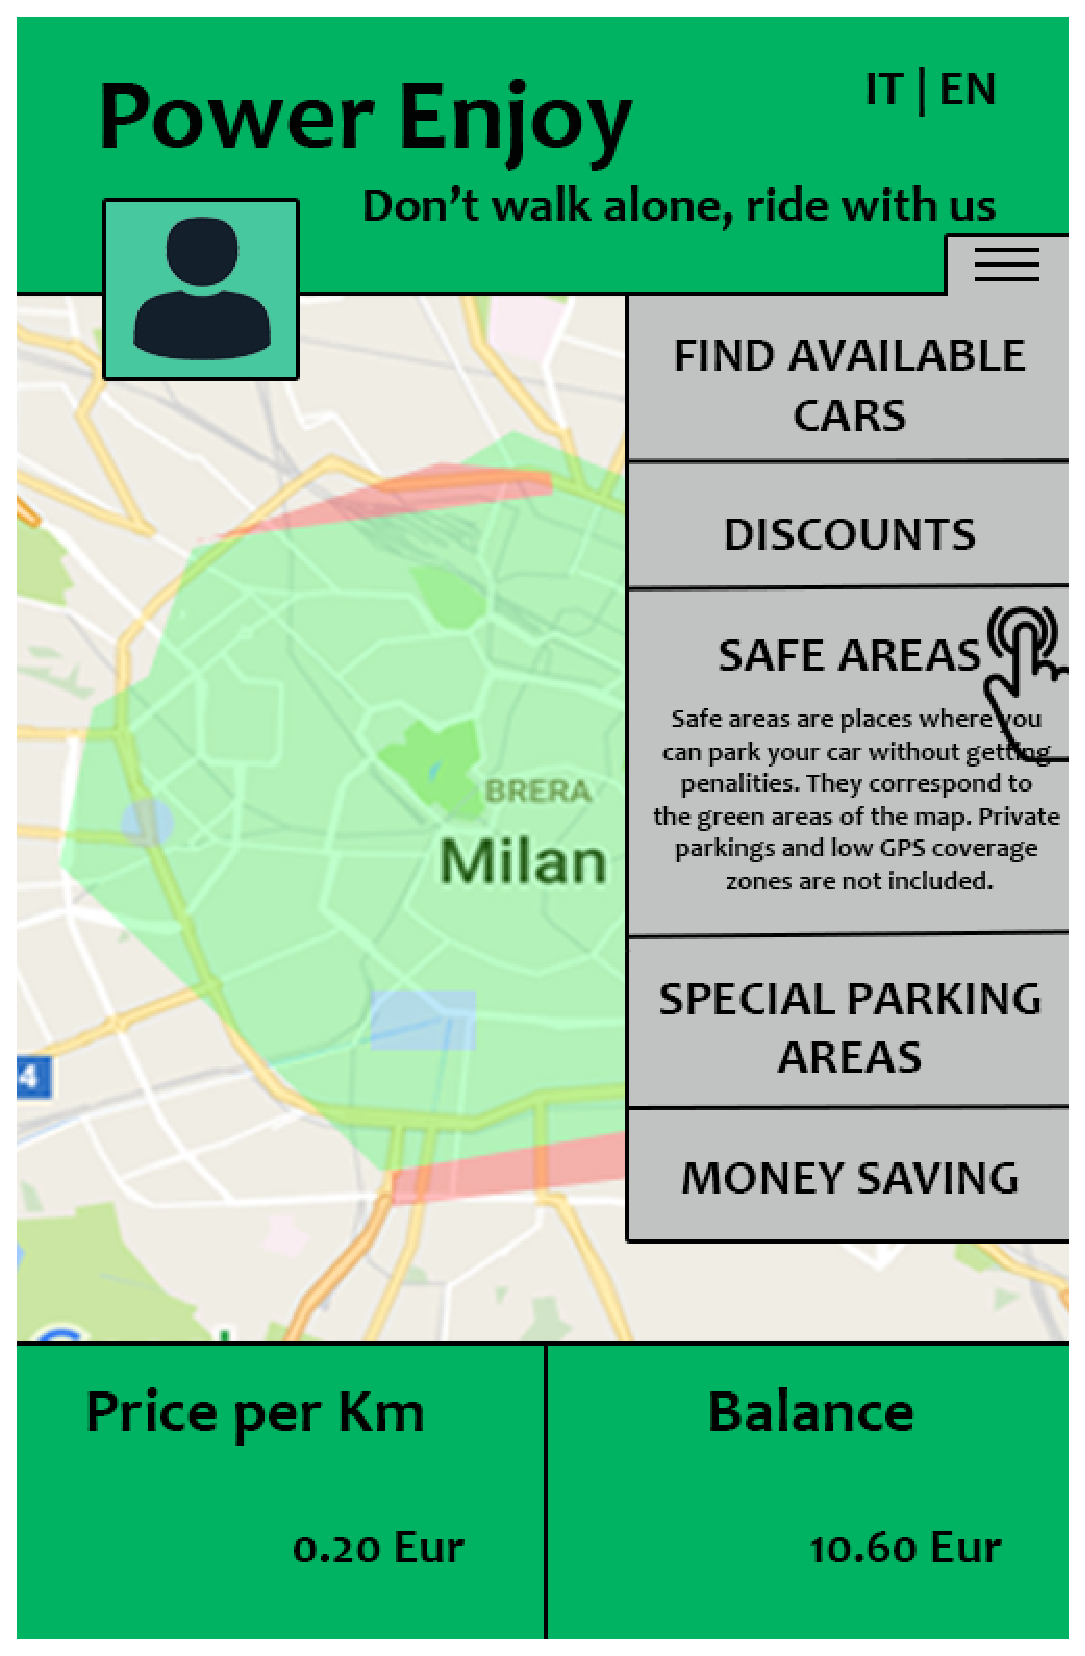
\includegraphics[height=4cm,keepaspectratio]{figures/mobile_logged.eps}
			\label{fig:mobile_logged}
			\textcolor{white}{\rule{\textwidth}{0cm}}
			\centering
			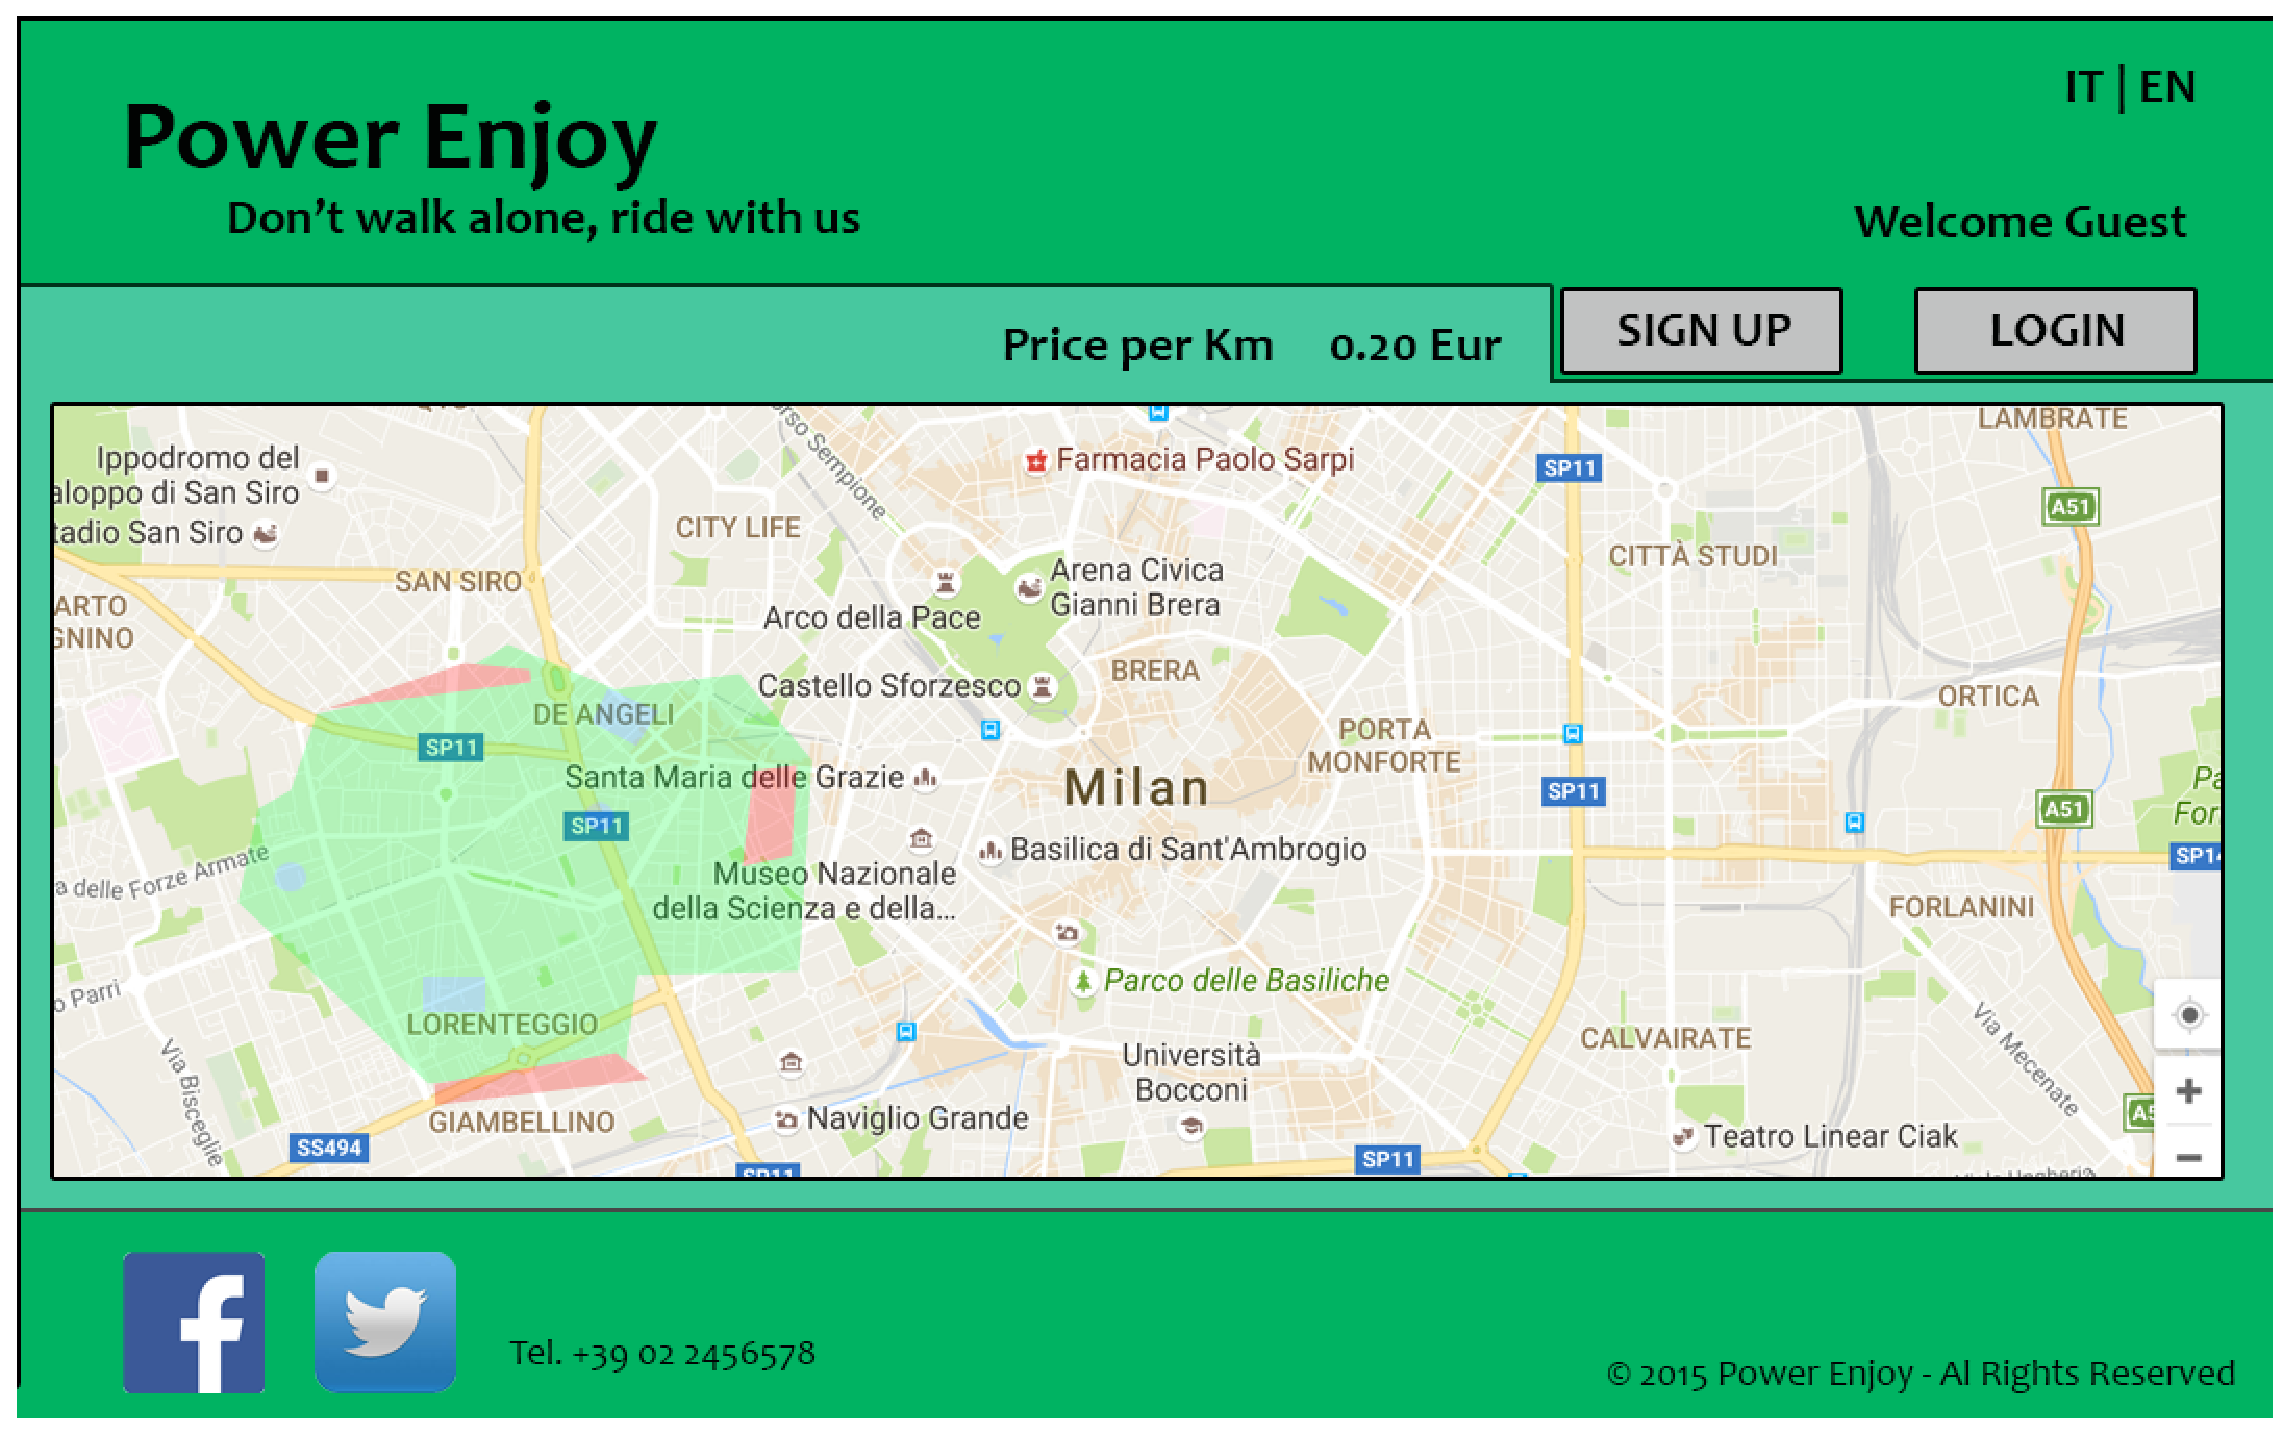
\includegraphics[width=4.7cm,keepaspectratio]{figures/desktop_unlogged.eps}
			\label{fig:desktop_unlogged}
		\end{figure}
	\end{columns}
\end{frame}

\begin{frame}
	\fontsize{7.5}{9}
	\begin{columns}[c]
		\column{.5\textwidth}
		Goals:
		\begin{itemize}
			\item \([\)G1] Registration of a user to the system
			\item \([\)G2] Finding the locations of the available cars
			\item \([\)G3] Reservation of a car
			\item \([\)G4] Expiration of reservation and penalization
			\item \([\)G5] Entry of registered user into the car
			\item \([\)G6] Start charging and notifying the registered user
			\item \([\)G7] Stop charging the registered user and lock the car
			\item \([\)G8] Safe areas for parking the reserved cars
			\item \([\)G9] Detection of extra passengers and applying discount
			\item \([\)G10] Detection of the battery status and applying discount
			\item \([\)G11] Detection of special parking areas and applying discount
			\item \([\)G12] Checking parking and battery constraints and penalization
		\end{itemize}
	
		\column{.45\textwidth}
		Domain properties:
		\begin{itemize}
			\item User's data are always valid.
			\item Location reported by the GPS is always accurate.
			\item Every user can reserve just a car per time.
			\item The service is only available to validated users.
			\item The service has employees to move the cars if their distribution in the map is unbalanced.
			\item The license office provides the online service to let the system instantly check the user's documents during the registration.
			\item If the user's driver license expires, he gets unvalidated until he renew it.
			\item A call center is provided by the service to handle difficult situations.
		\end{itemize}
	\end{columns}
\end{frame}

\begin{frame}
	\fontsize{7.5}{9}
	\frametitle{Requirements}
	\begin{itemize}
		\item The system needs to provide mandatory sign up and payment options or the guest users who wants to register to use the car sharing service.
		\item Once the payment is successful and the guest user is registered, the registered user receives a password that can be used to access (login into) the system.
		\item The system needs to provide the exact location of the cars that are available within a certain distance either from the current location of the registered users or from a specified address given(entered) by the registered users.
		\item The system provides provision such that the registered users must be able to reserve only a single car among the available cars in a certain geographical region for up to one hour before they pick it up.
		\item The system checks if a reserved car is picked-up within one hour. If not, the system tags the car as available again and the reservation expires.
		\item The system penalizes the registered user who made the reservation and did not pick the reserved car within an hour, by making him to pay a fee of 1EUR.
	\end{itemize}
	
	\vspace*{-0.3cm}
	\begin{figure}[H]
		\centering
		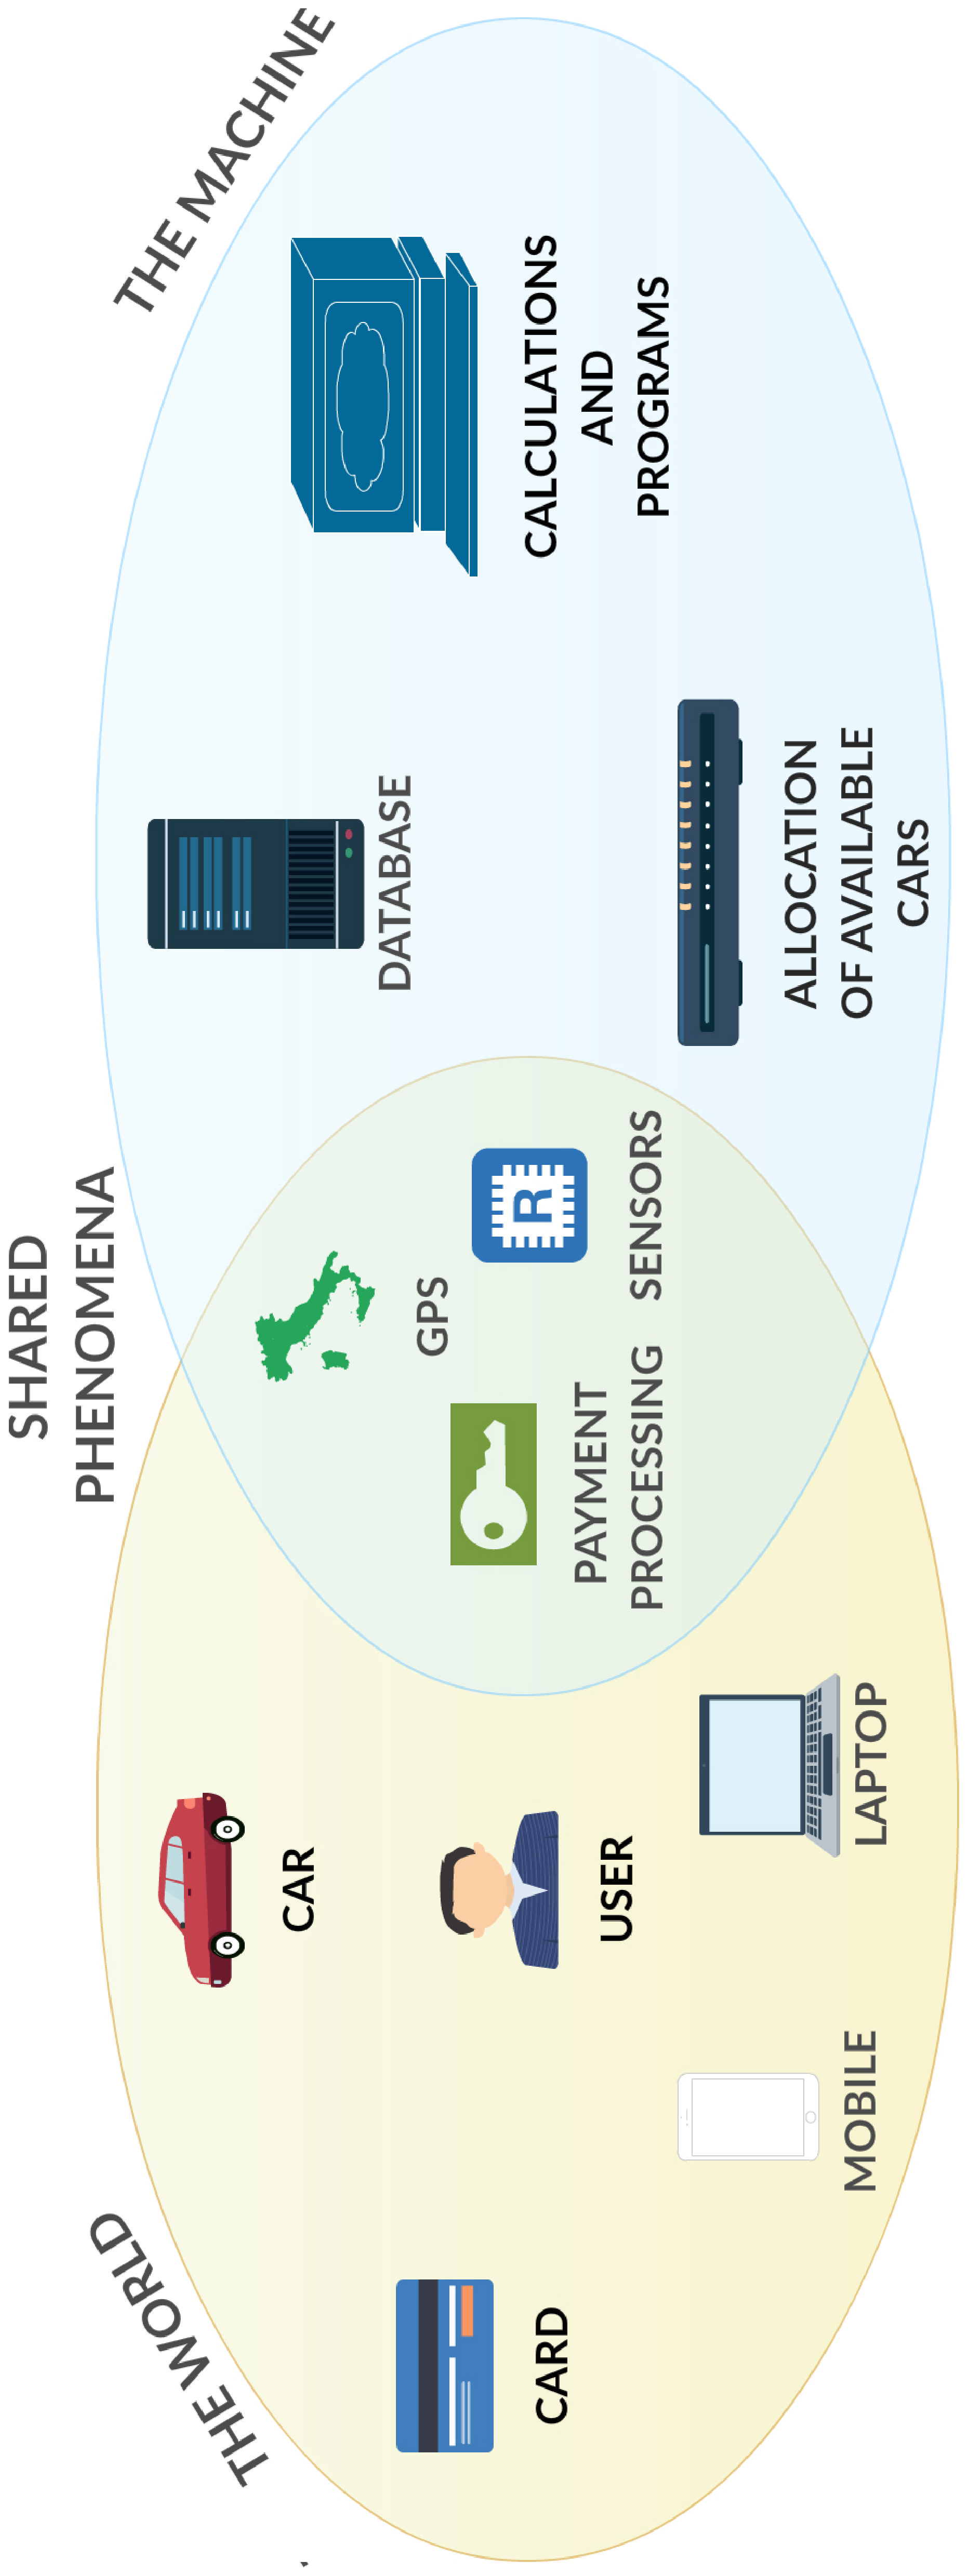
\includegraphics[width=3.3cm,keepaspectratio,angle=270]{figures/world_and_machine.eps}
		\label{fig:world_and_machine}
	\end{figure}
\end{frame}

\begin{frame}
	\frametitle{UML Model - Use Case Diagram}
	\begin{figure}[H]
		\centering
		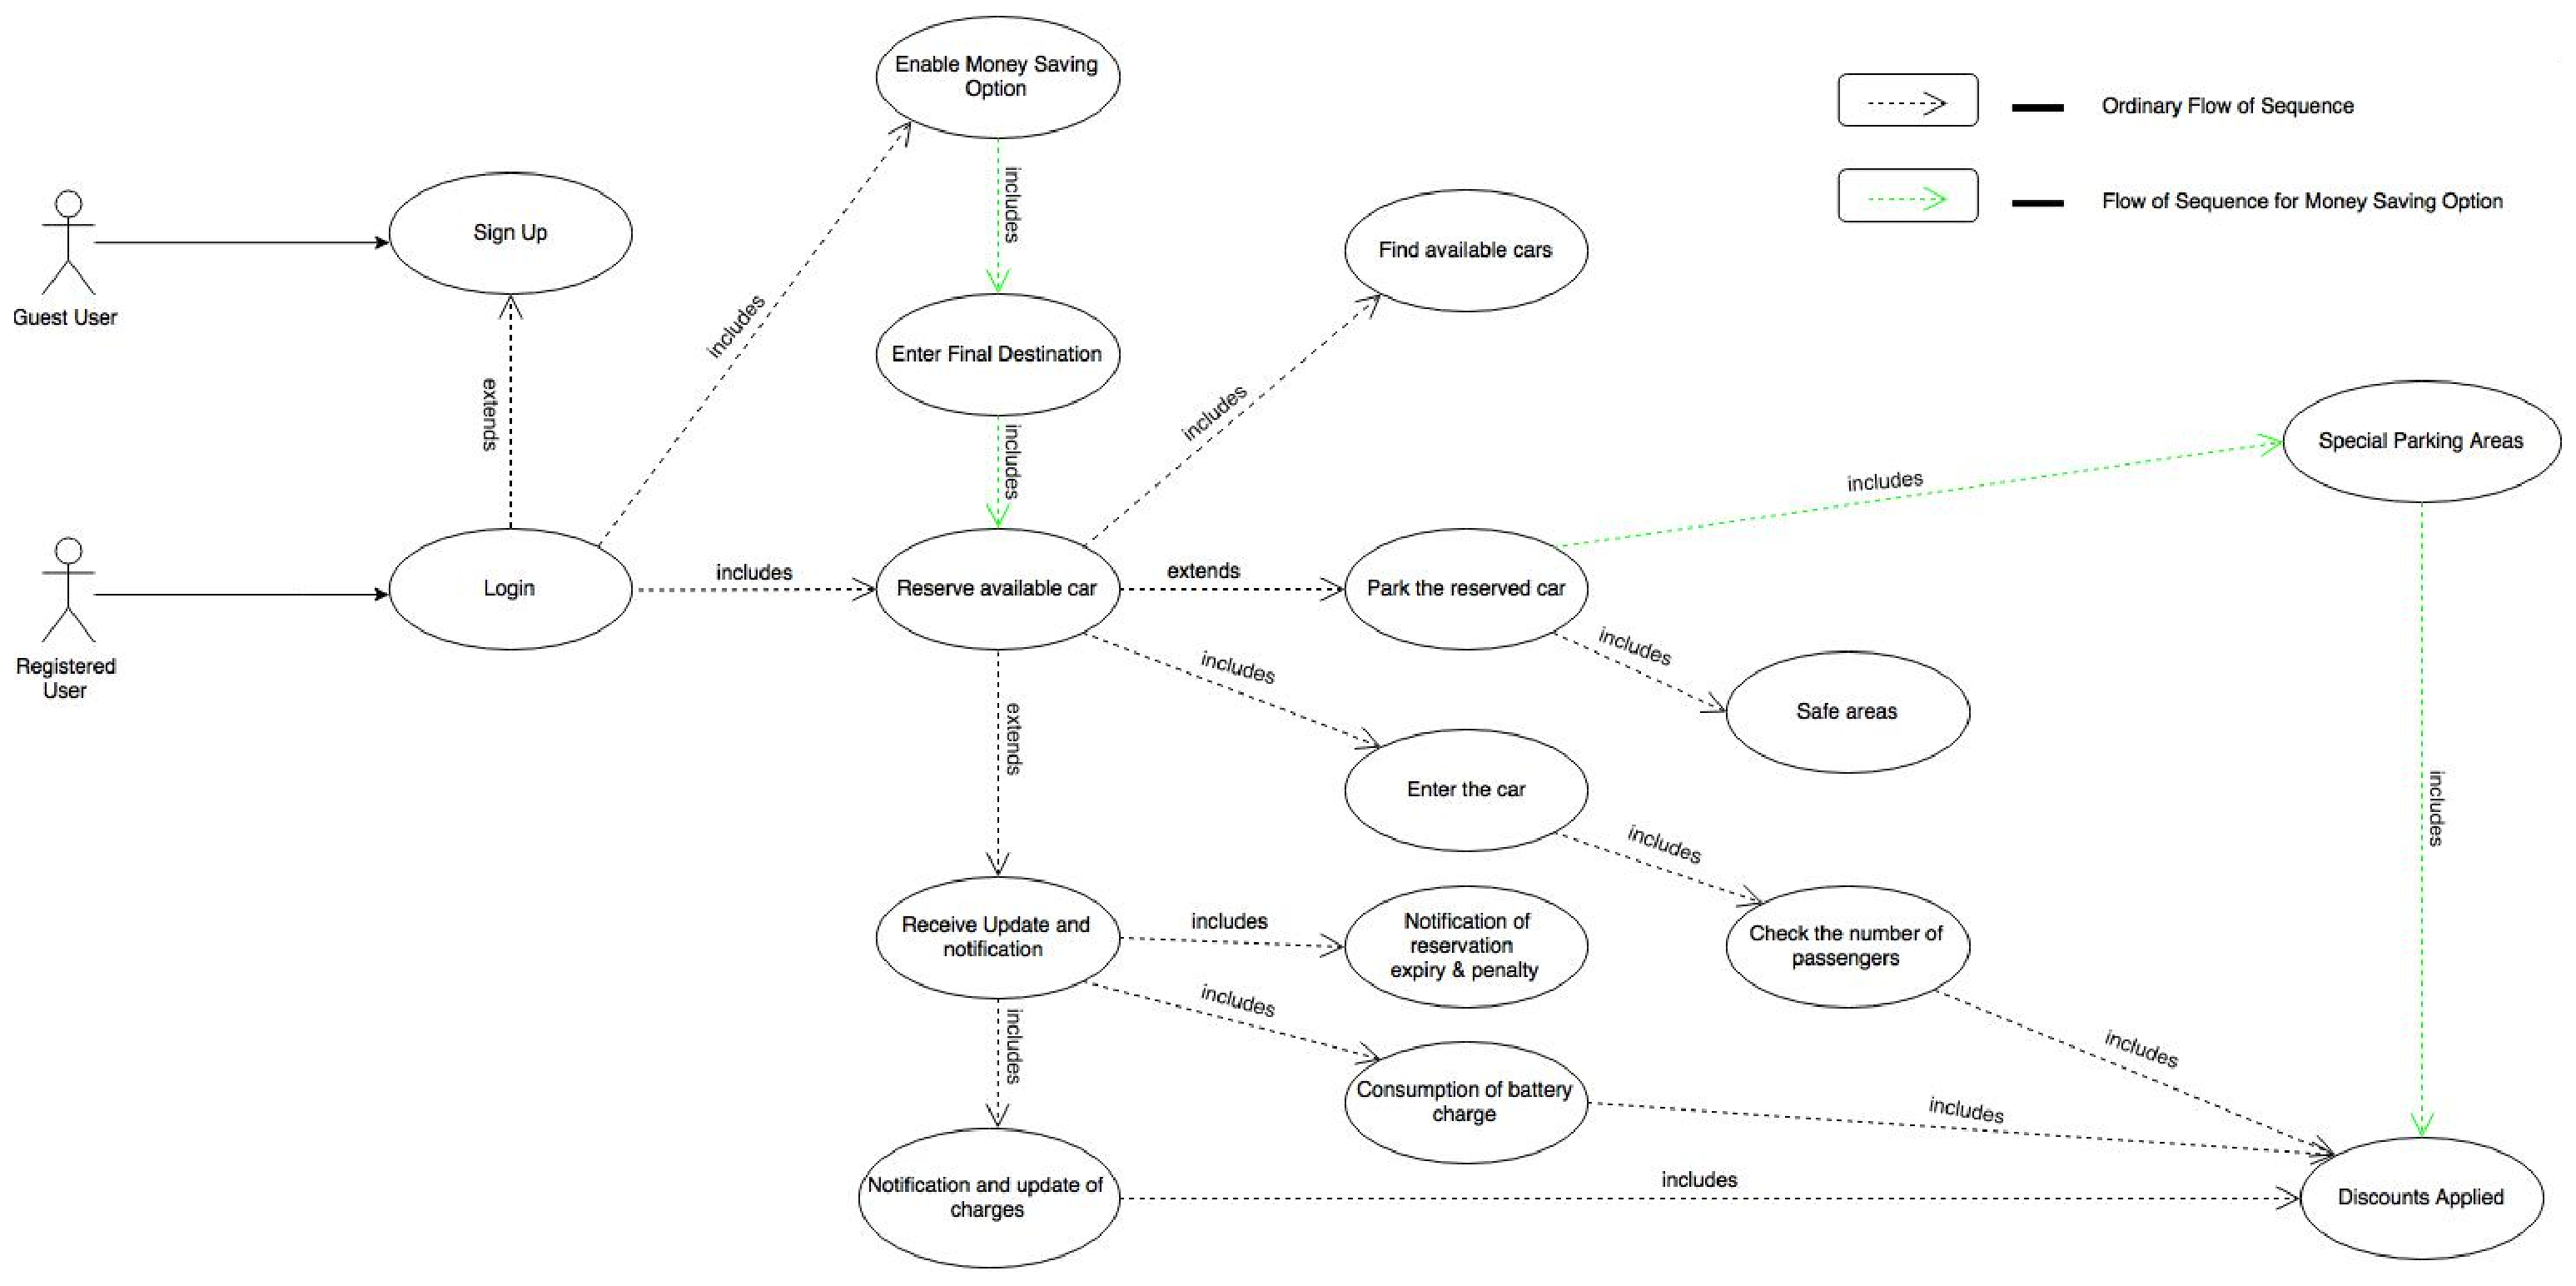
\includegraphics[width=\linewidth,keepaspectratio]{figures/use_case_diagram.eps}
		\label{fig:use_case_diagram}
	\end{figure}
\end{frame}

\begin{frame}
	\frametitle{UML Model - Sequence Diagrams}
	\begin{columns}[c]
		\column{.5\textwidth}
		\begin{figure}[H]
			\centering
			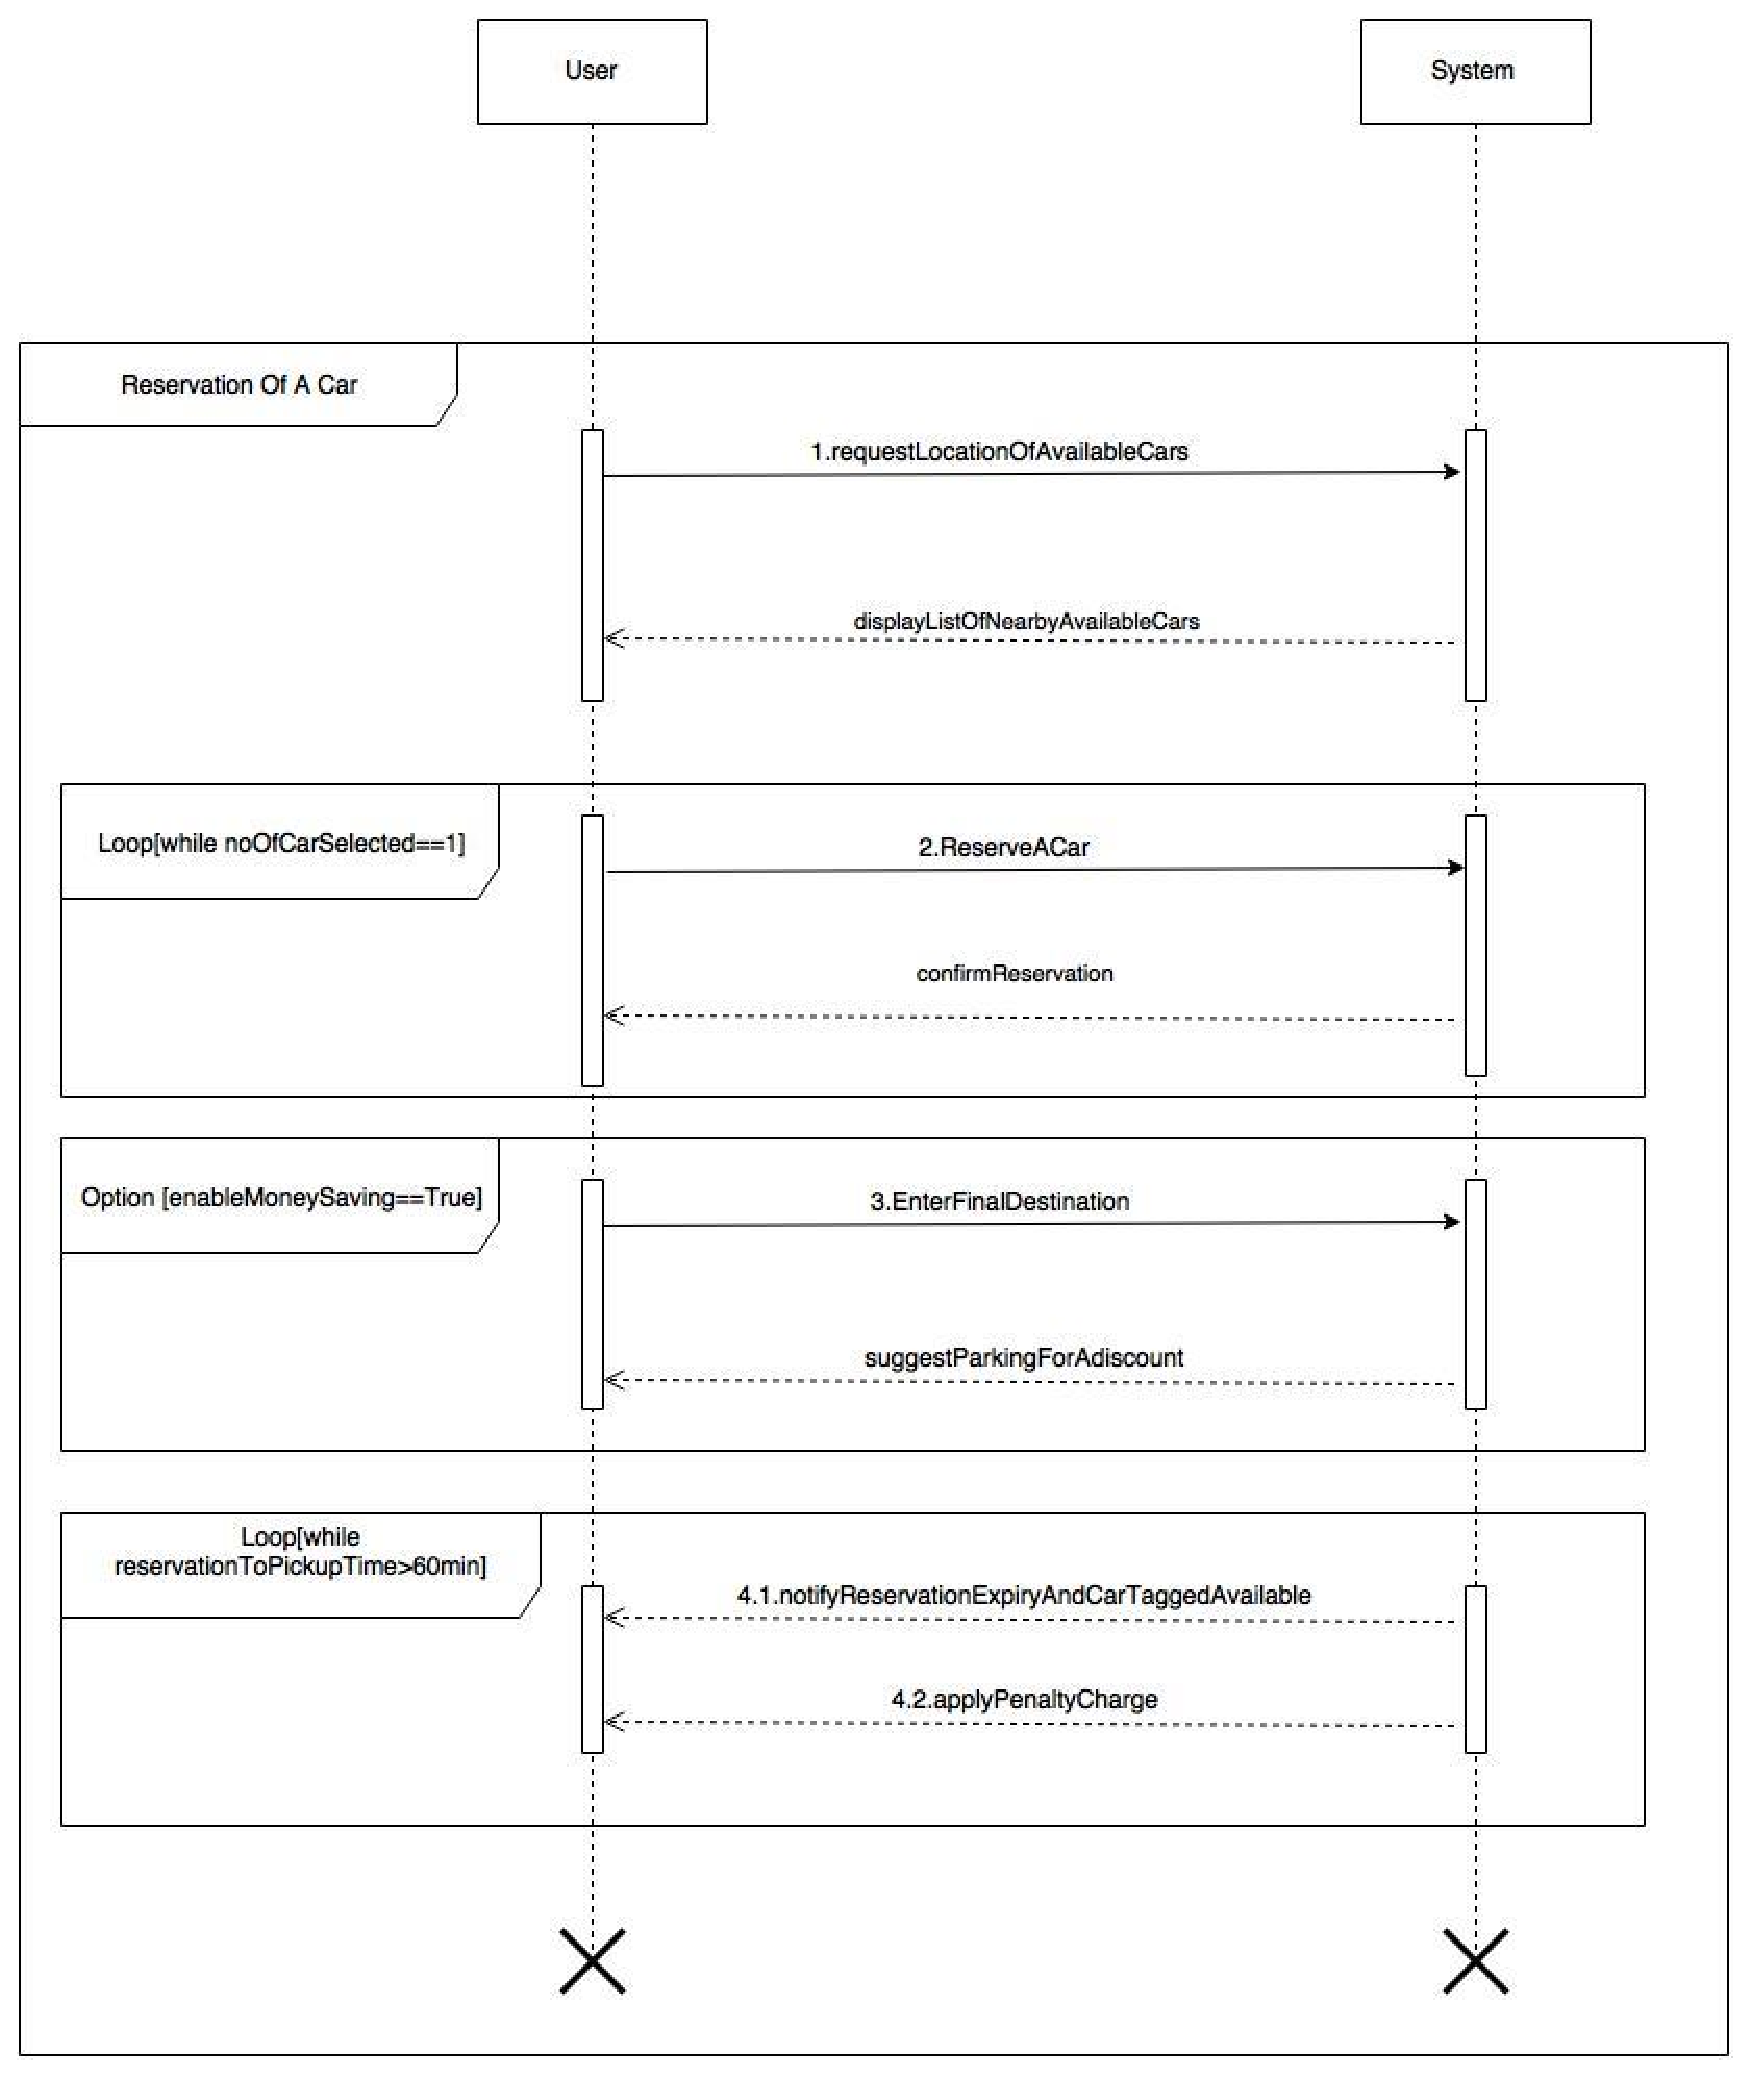
\includegraphics[height=6.7cm,keepaspectratio]{figures/sequence_reservation.eps}
			\label{fig:sequence_reservation}
		\end{figure}
		\column{.5\textwidth}
		\begin{figure}[H]
			\centering
			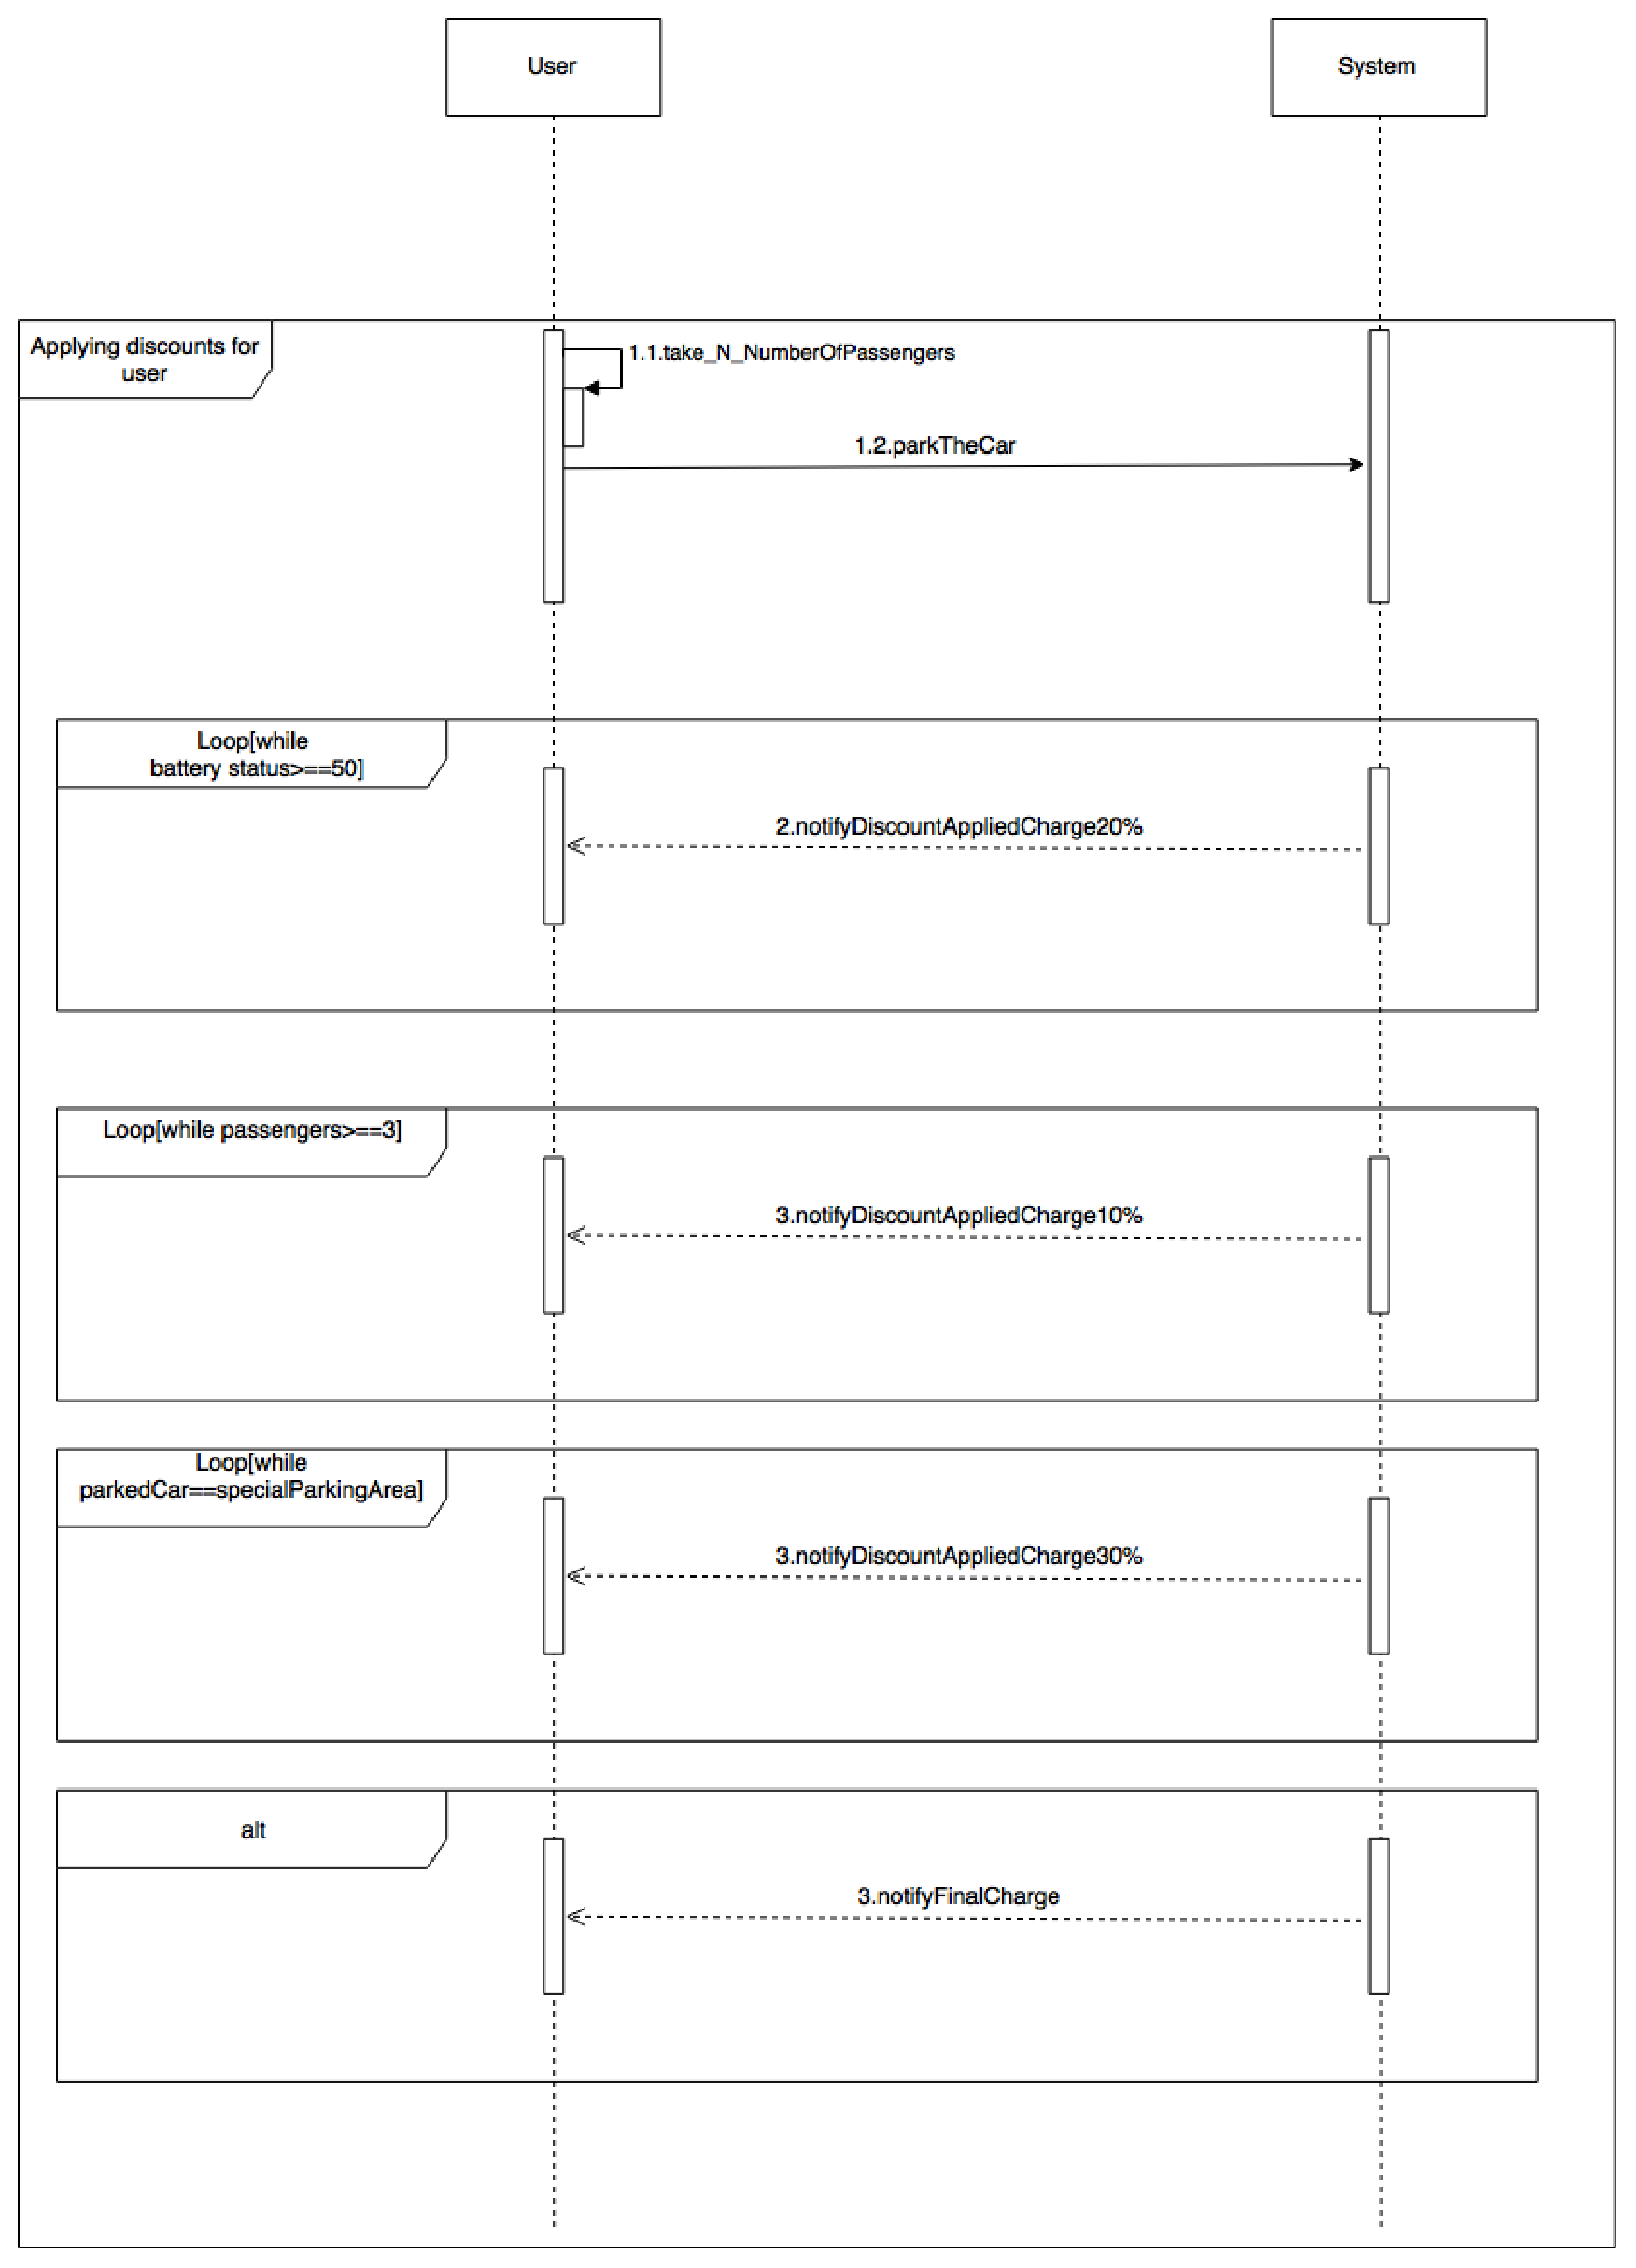
\includegraphics[height=7.5cm,keepaspectratio]{figures/sequence_discounts.eps}
			\label{fig:sequence_discounts}
		\end{figure}
	\end{columns}
\end{frame}

\begin{frame}
	\frametitle{UML Model - Class Diagram}
	\begin{figure}[H]
		\centering
		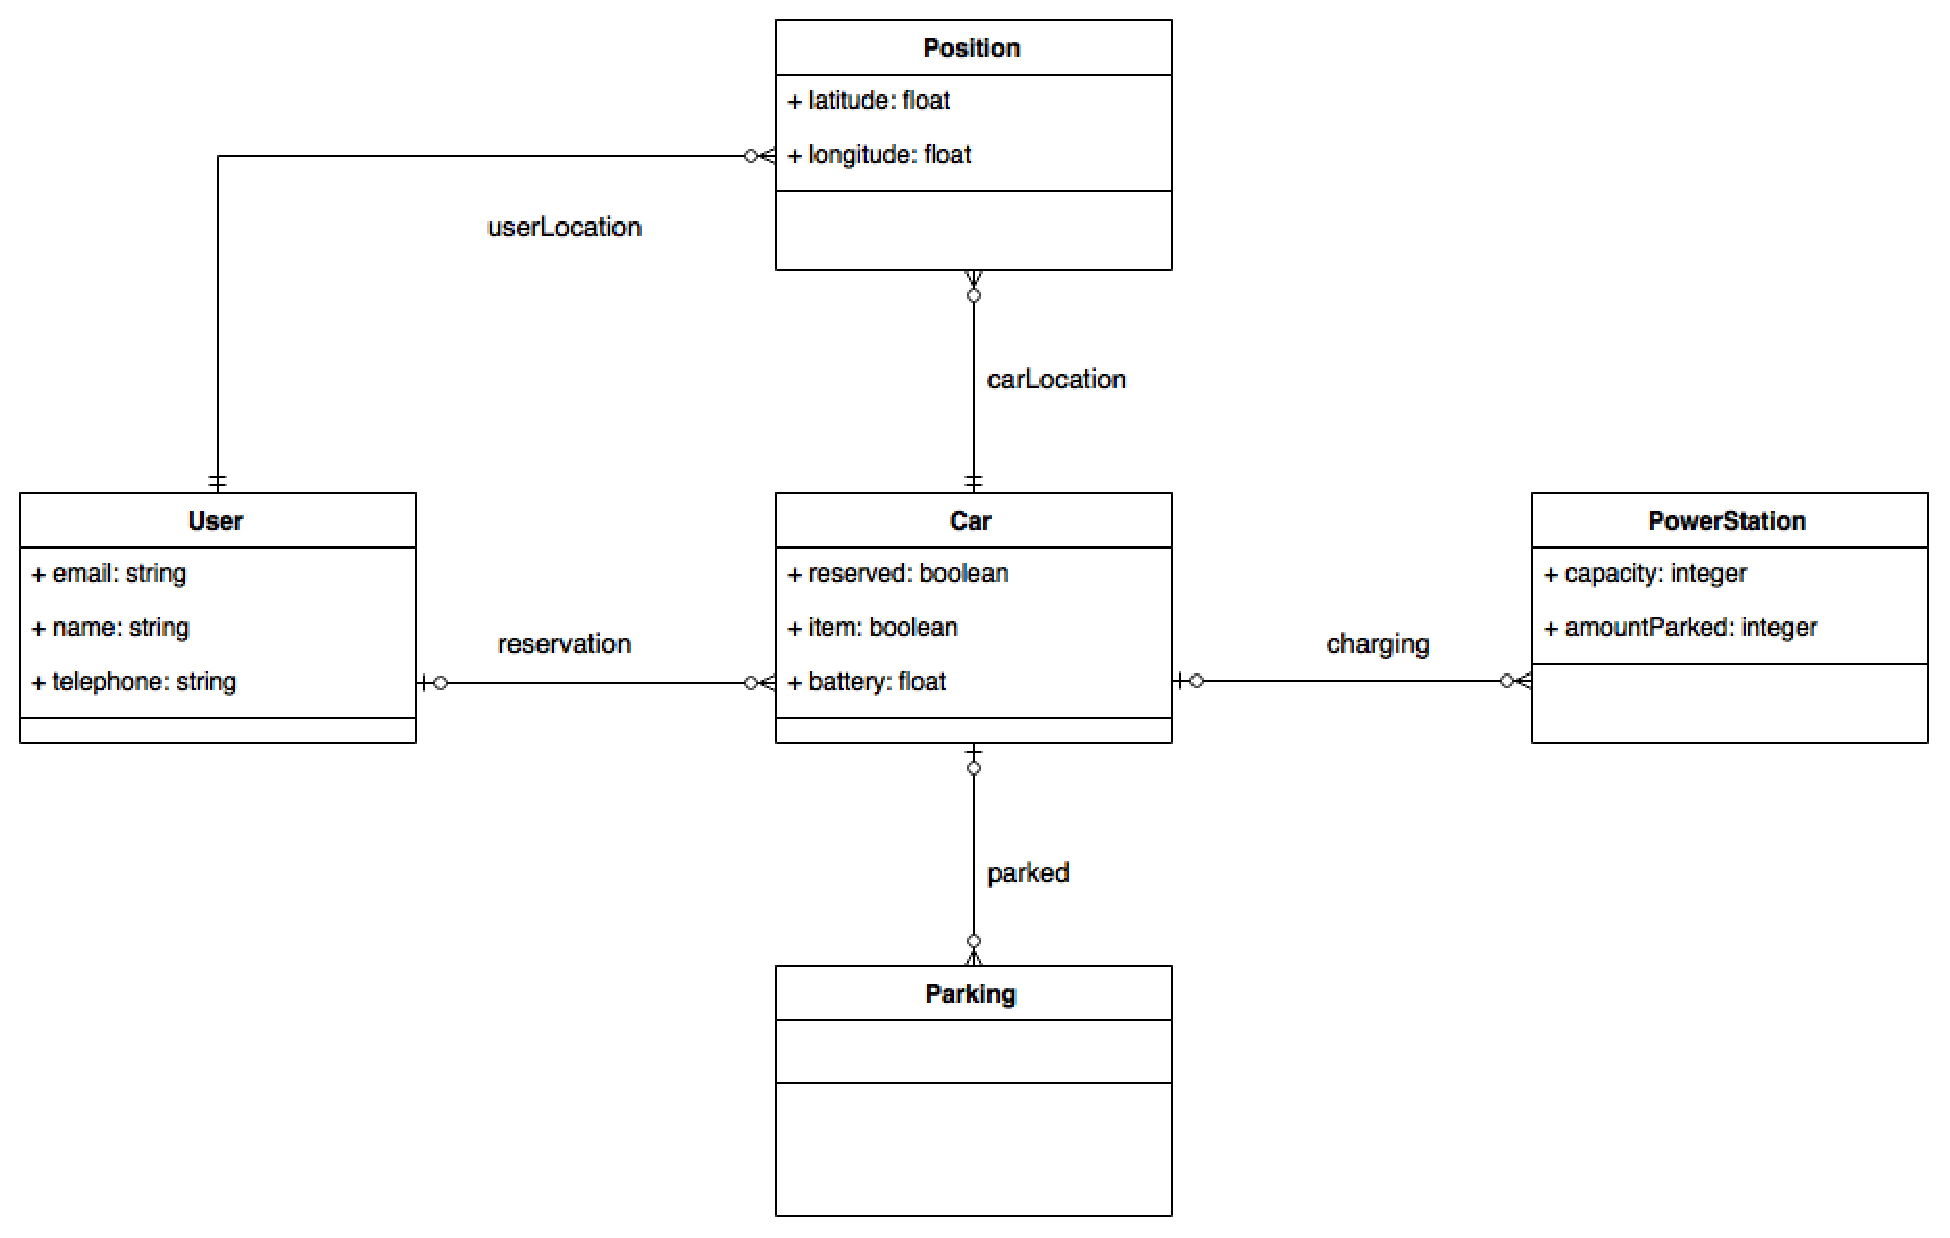
\includegraphics[height=7.3cm,keepaspectratio]{figures/class_diagram.eps}
		\label{fig:class_diagram}
	\end{figure}
\end{frame}

\begin{frame}
	\frametitle{UML Model - Activity Diagrams}
	\begin{columns}[c]
		\column{.5\textwidth}
		\begin{figure}[H]
			\centering
			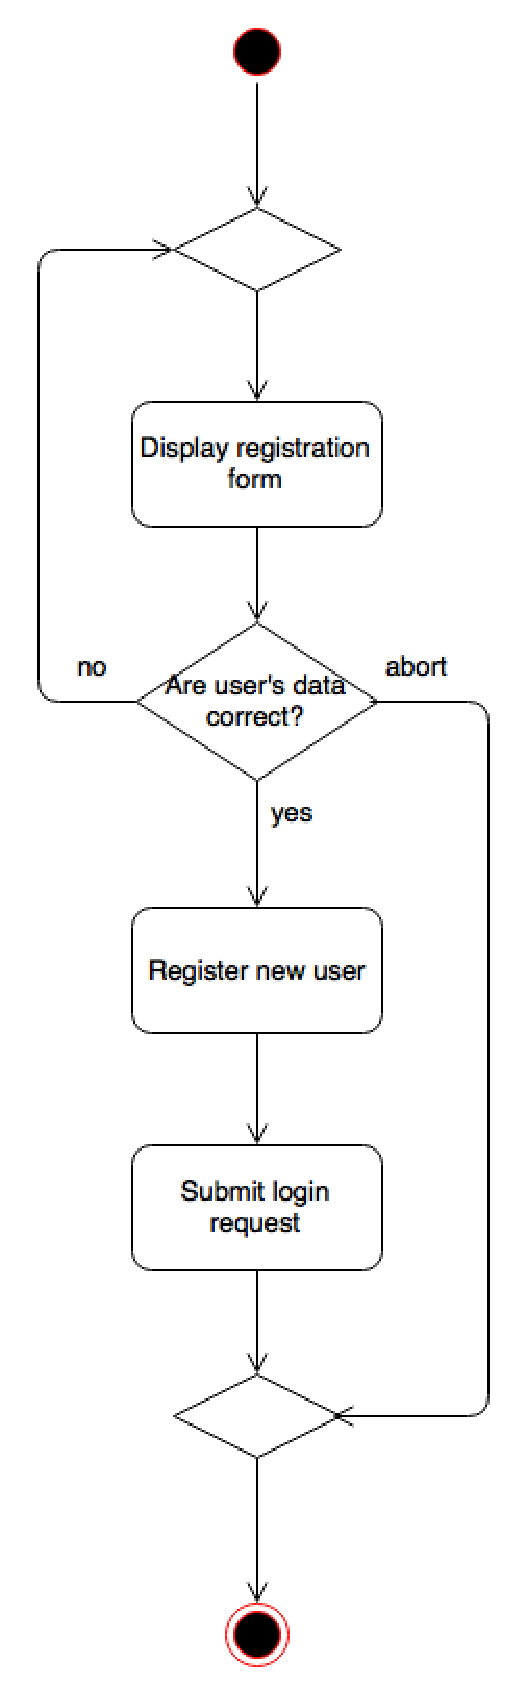
\includegraphics[height=6.9cm,keepaspectratio]{figures/registration_activity_diagram.eps}
			\label{fig:registration_activity_diagram}
		\end{figure}
		\column{.5\textwidth}
		\begin{figure}[H]
			\centering
			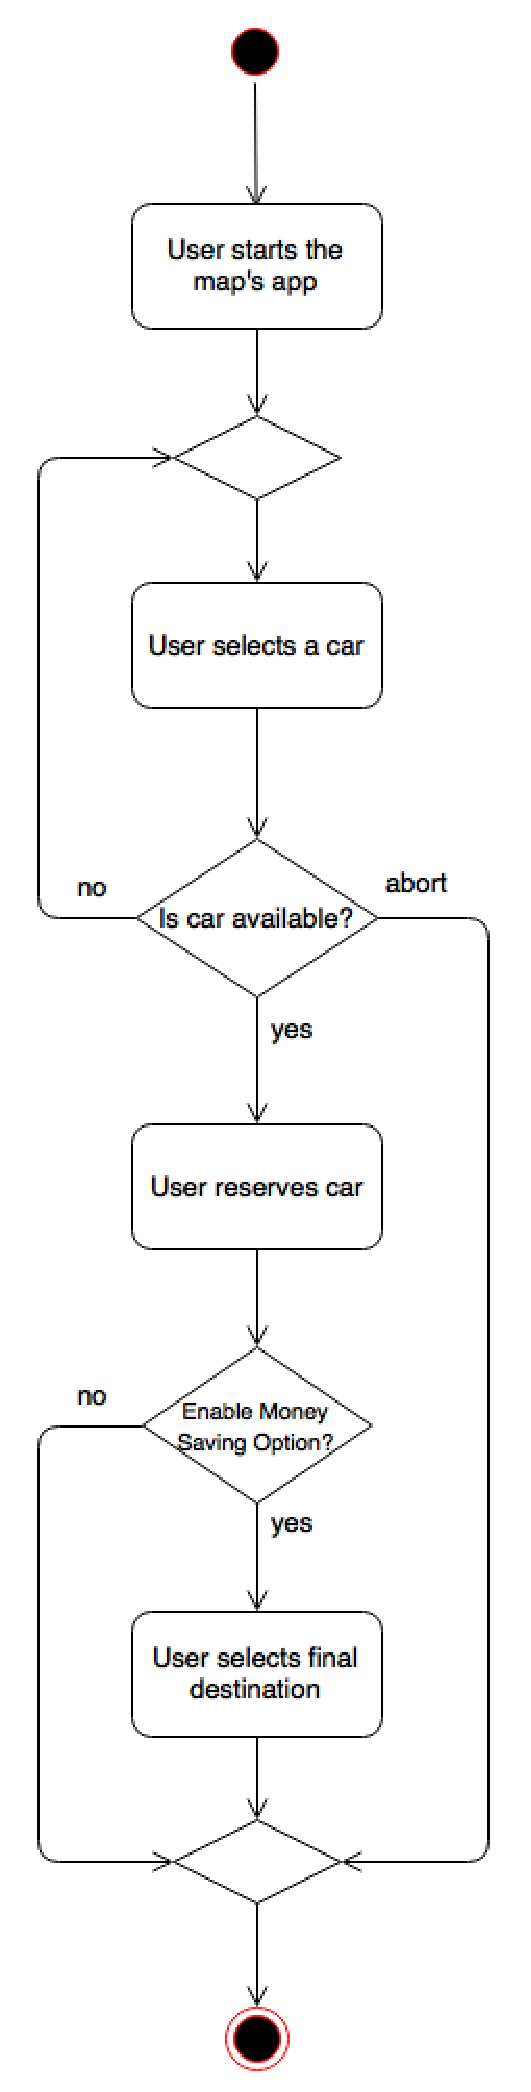
\includegraphics[height=7.6cm,keepaspectratio]{figures/reservation_activity_diagram.eps}
			\label{fig:reservation_activity_diagram}
		\end{figure}
	\end{columns}
\end{frame}

\begin{frame}
	\frametitle{Alloy Model and World Generated}
	\begin{figure}[H]
		\centering
		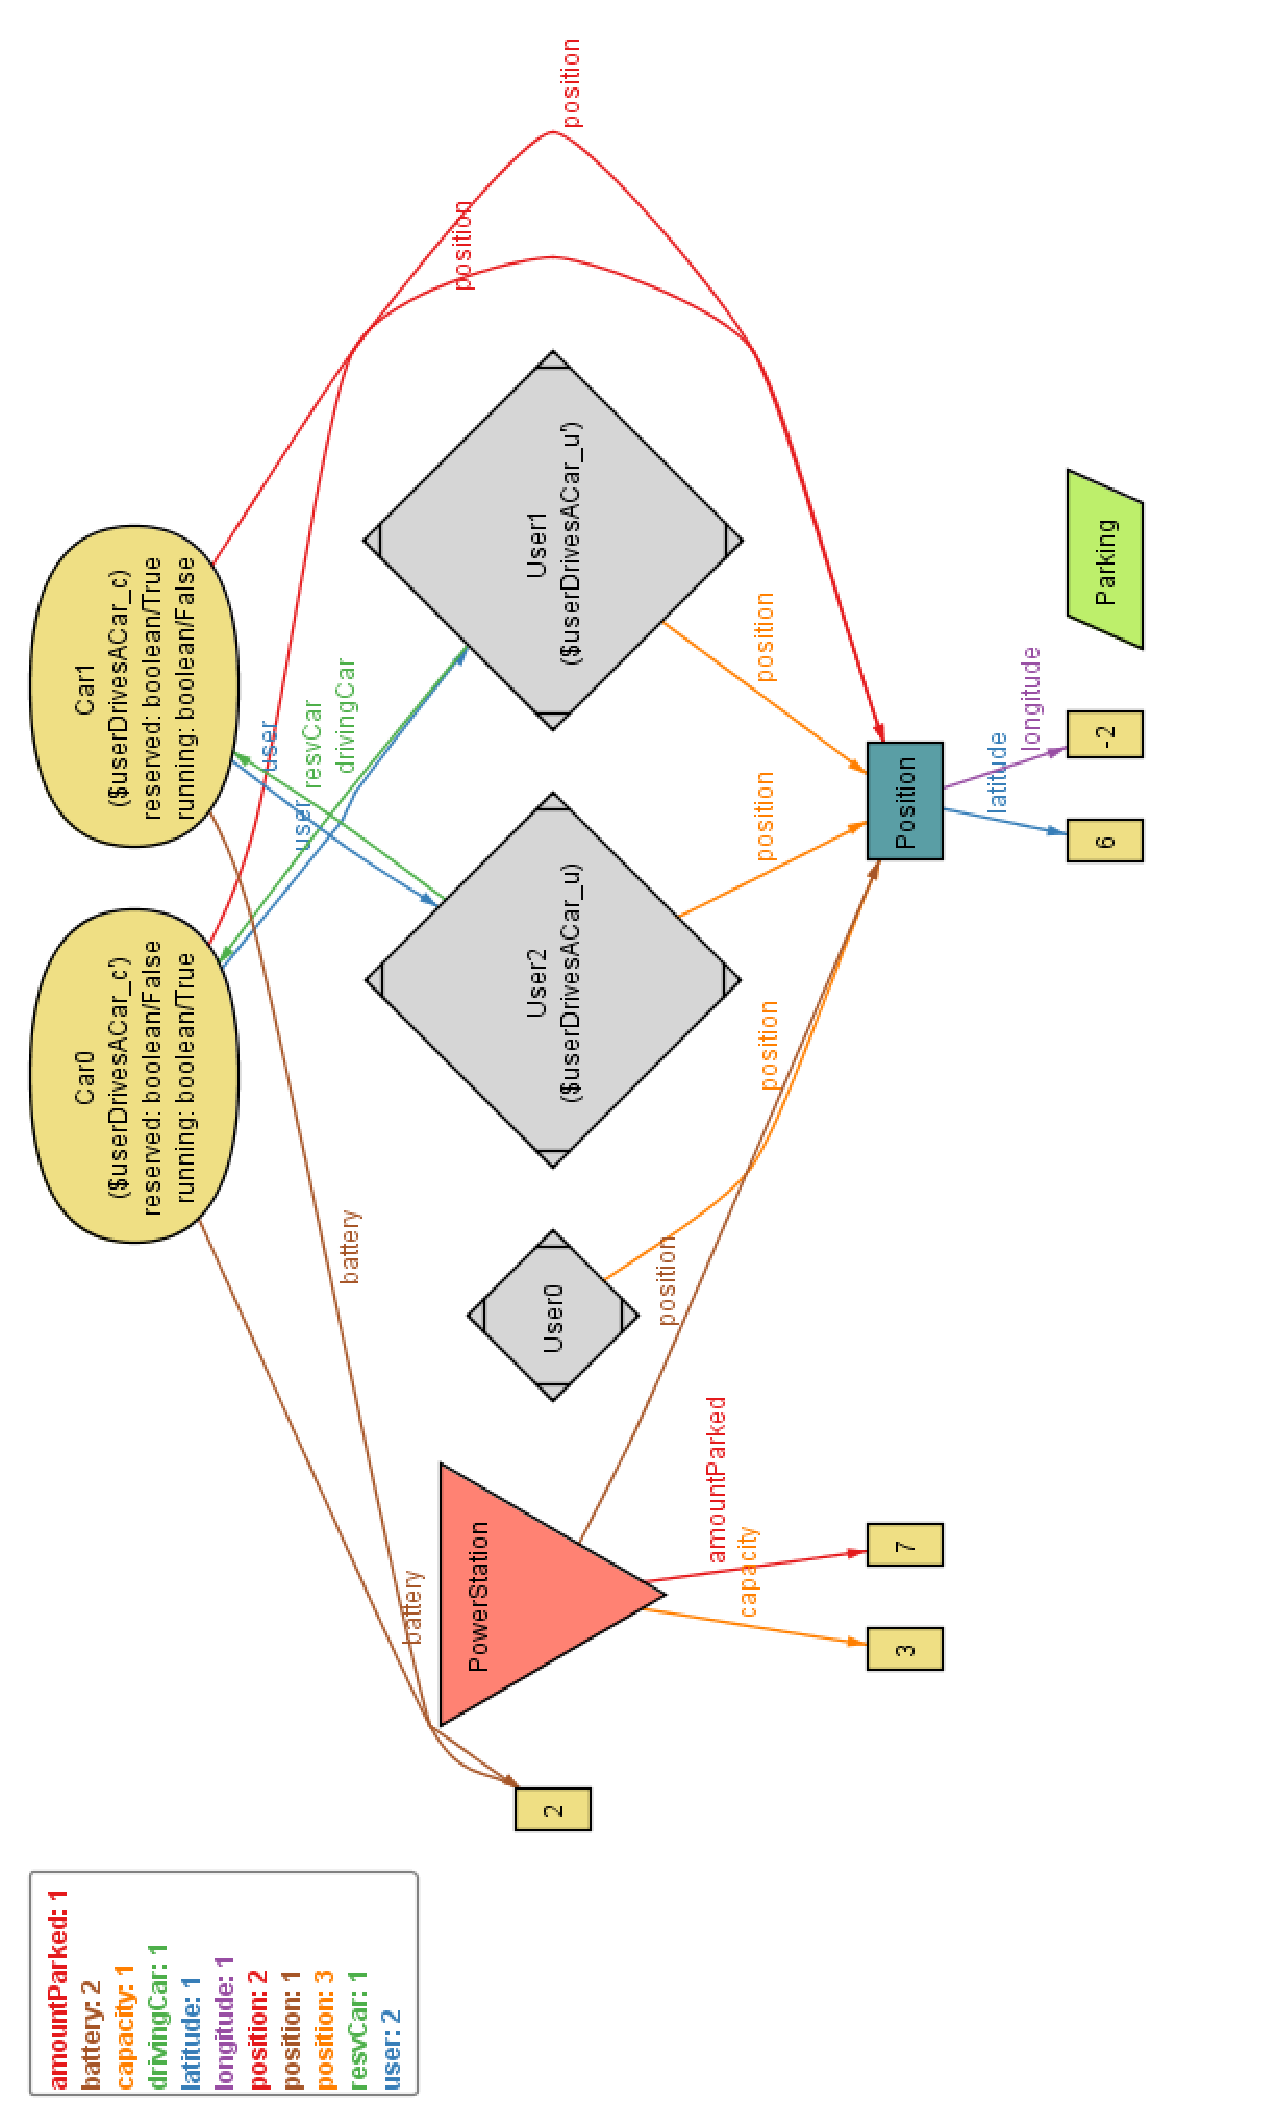
\includegraphics[width=7.3cm,keepaspectratio, angle=270]{figures/world_generated_driving.eps}
		\label{fig:world_generated_driving}
	\end{figure}
\end{frame}

\end{document}

\section{Design Document}

\begin{frame}
	\frametitle{Three-tier Architecture}
	\begin{figure}[H]
		\centering
		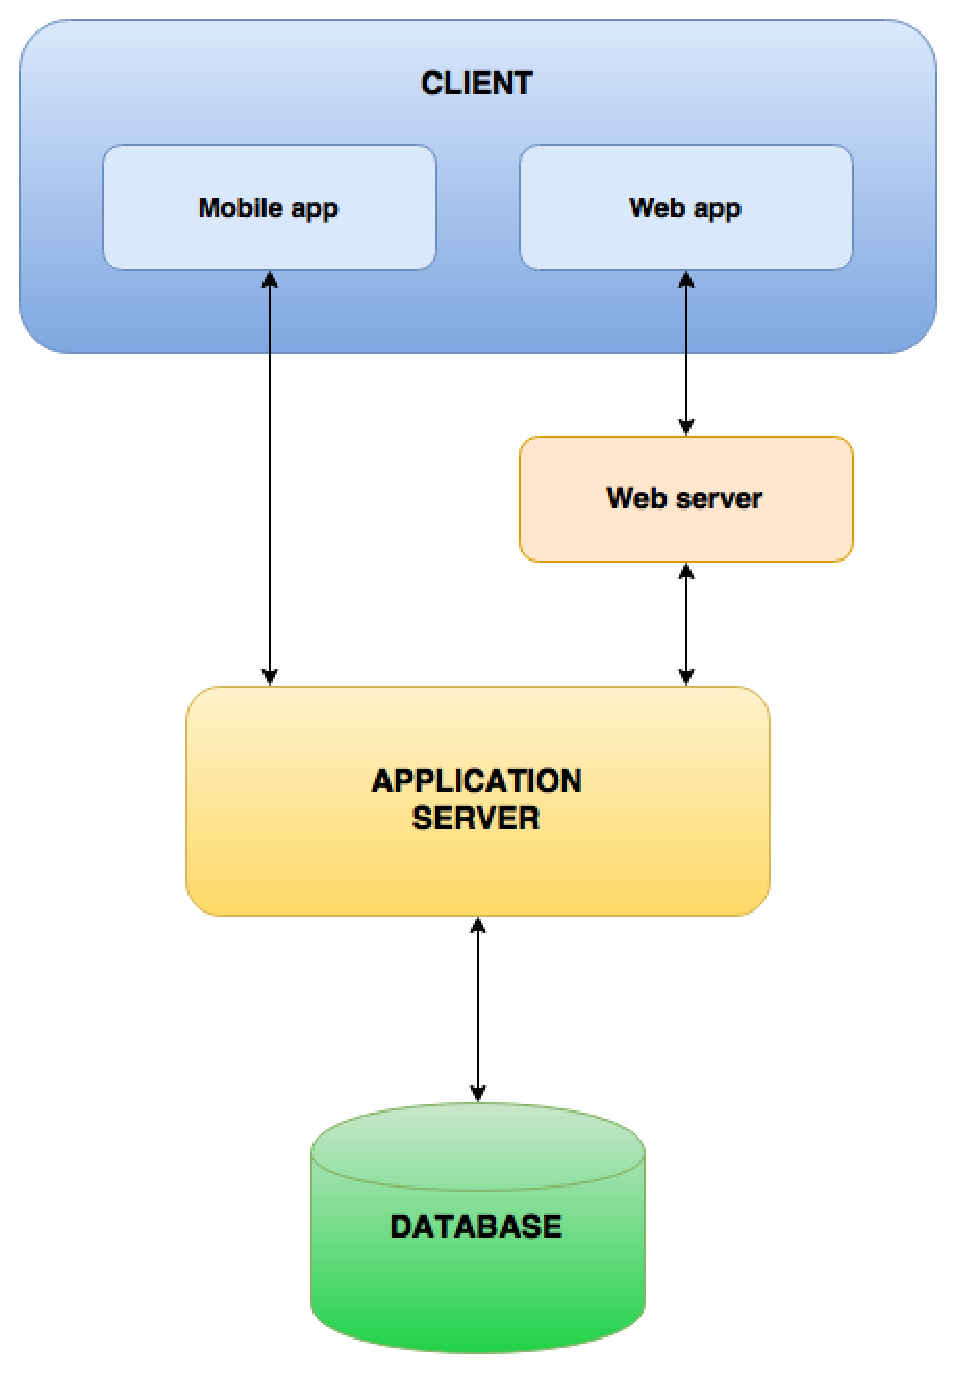
\includegraphics[height=7.3cm,keepaspectratio]{figures/layers.eps}
		\label{fig:layers}
	\end{figure}
\end{frame}

\begin{frame}
	\frametitle{Component View}
	\begin{figure}[H]
		\vspace*{-0.5cm}
		\centering
		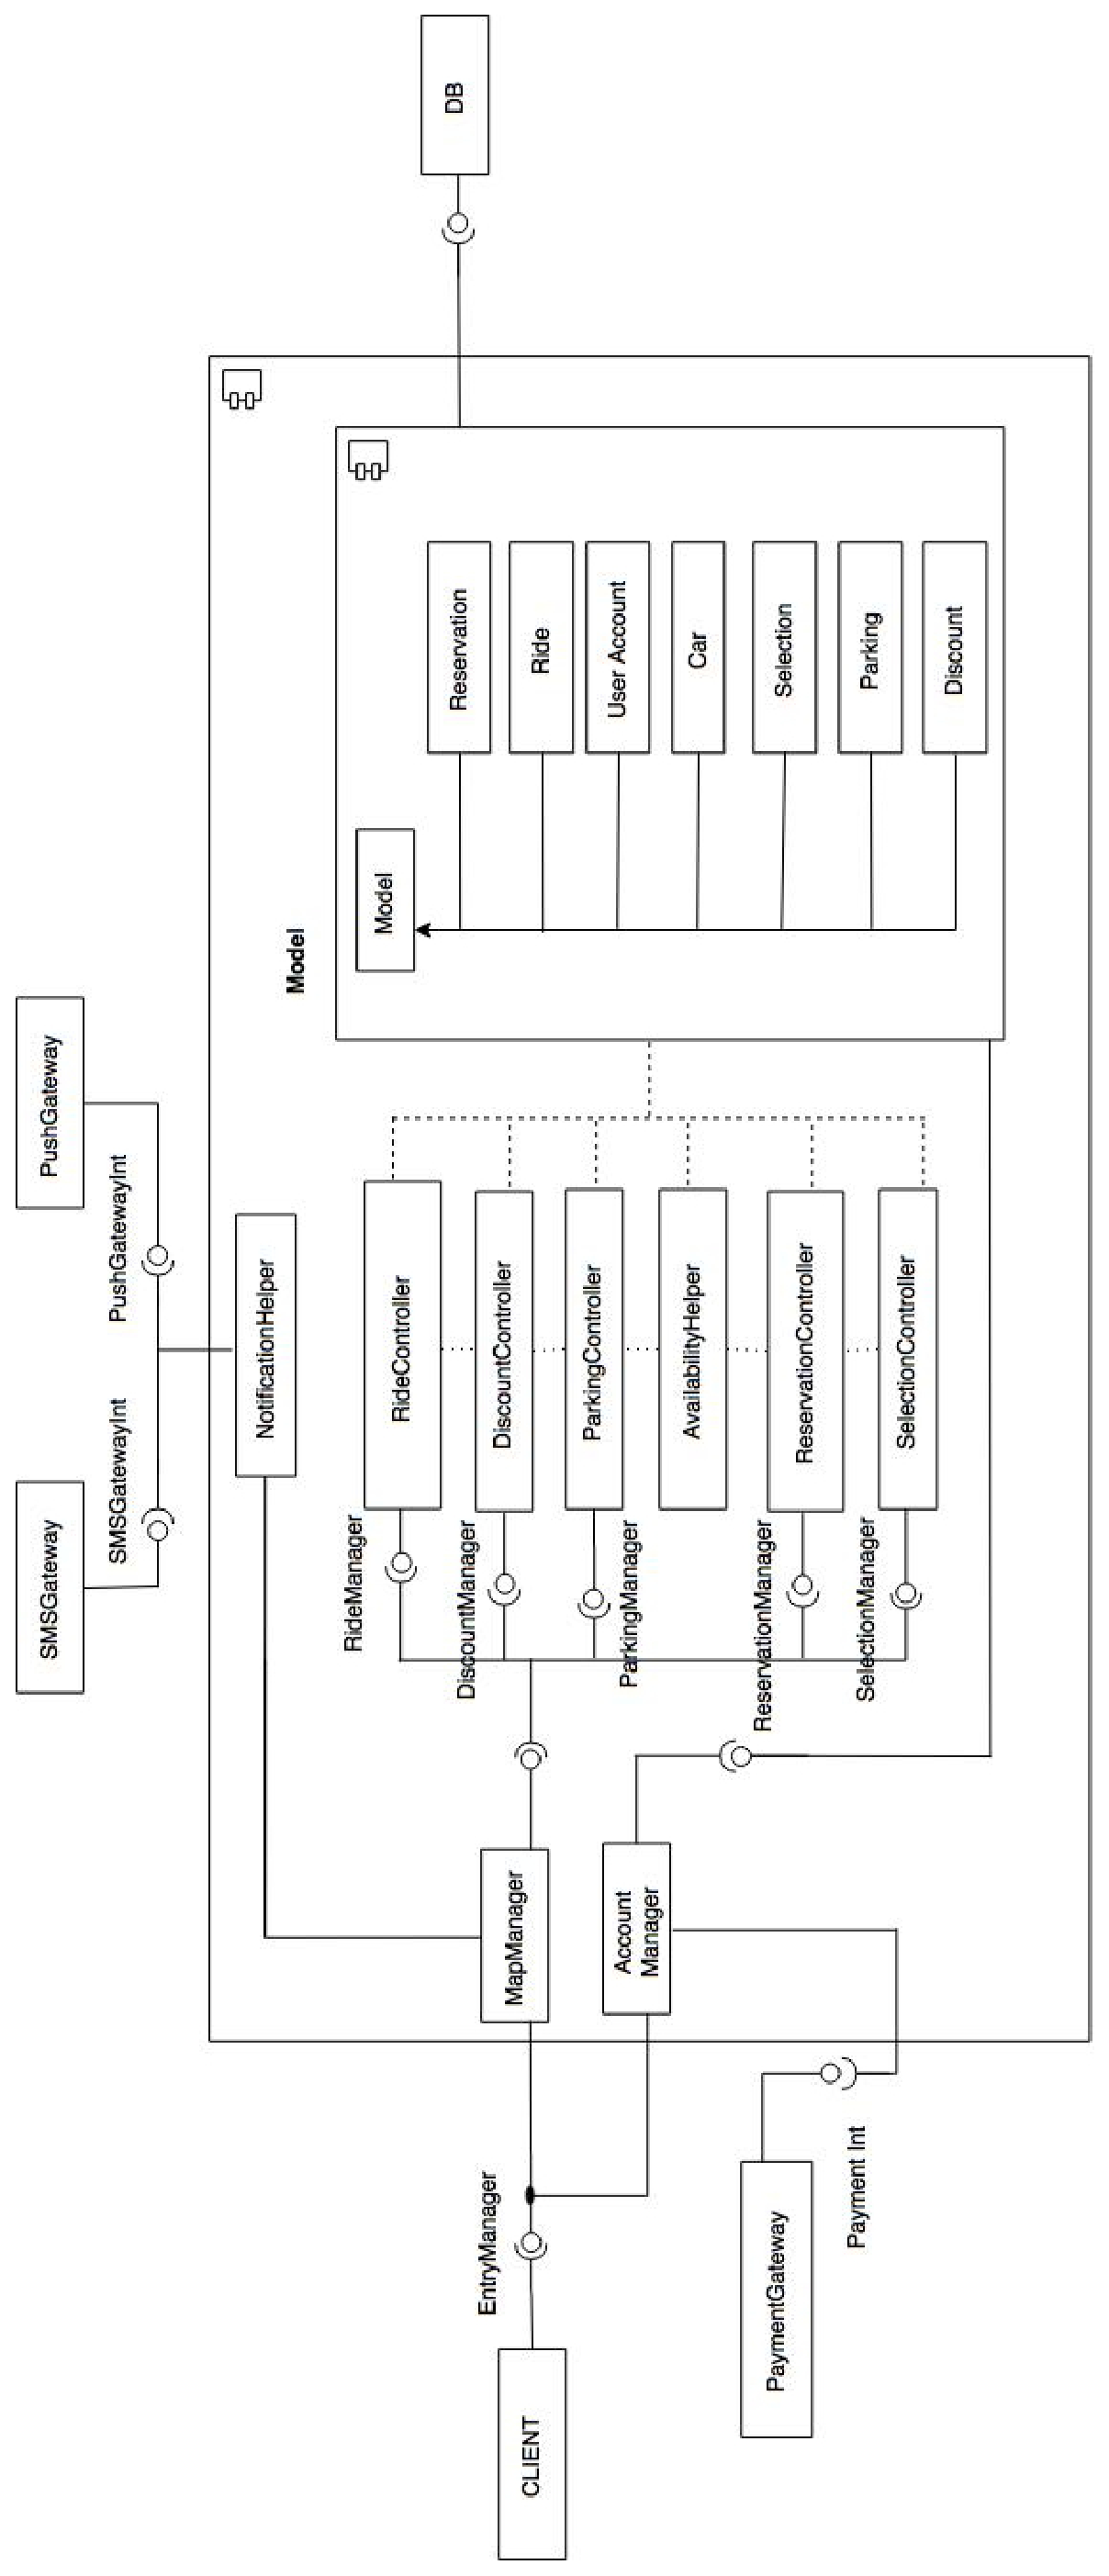
\includegraphics[height=12cm,keepaspectratio,angle=270]{figures/component_view.eps}
		\label{fig:component_view}
	\end{figure}
\end{frame}

\begin{frame}
	\frametitle{Deployment View}
	\begin{figure}[H]
		\centering
		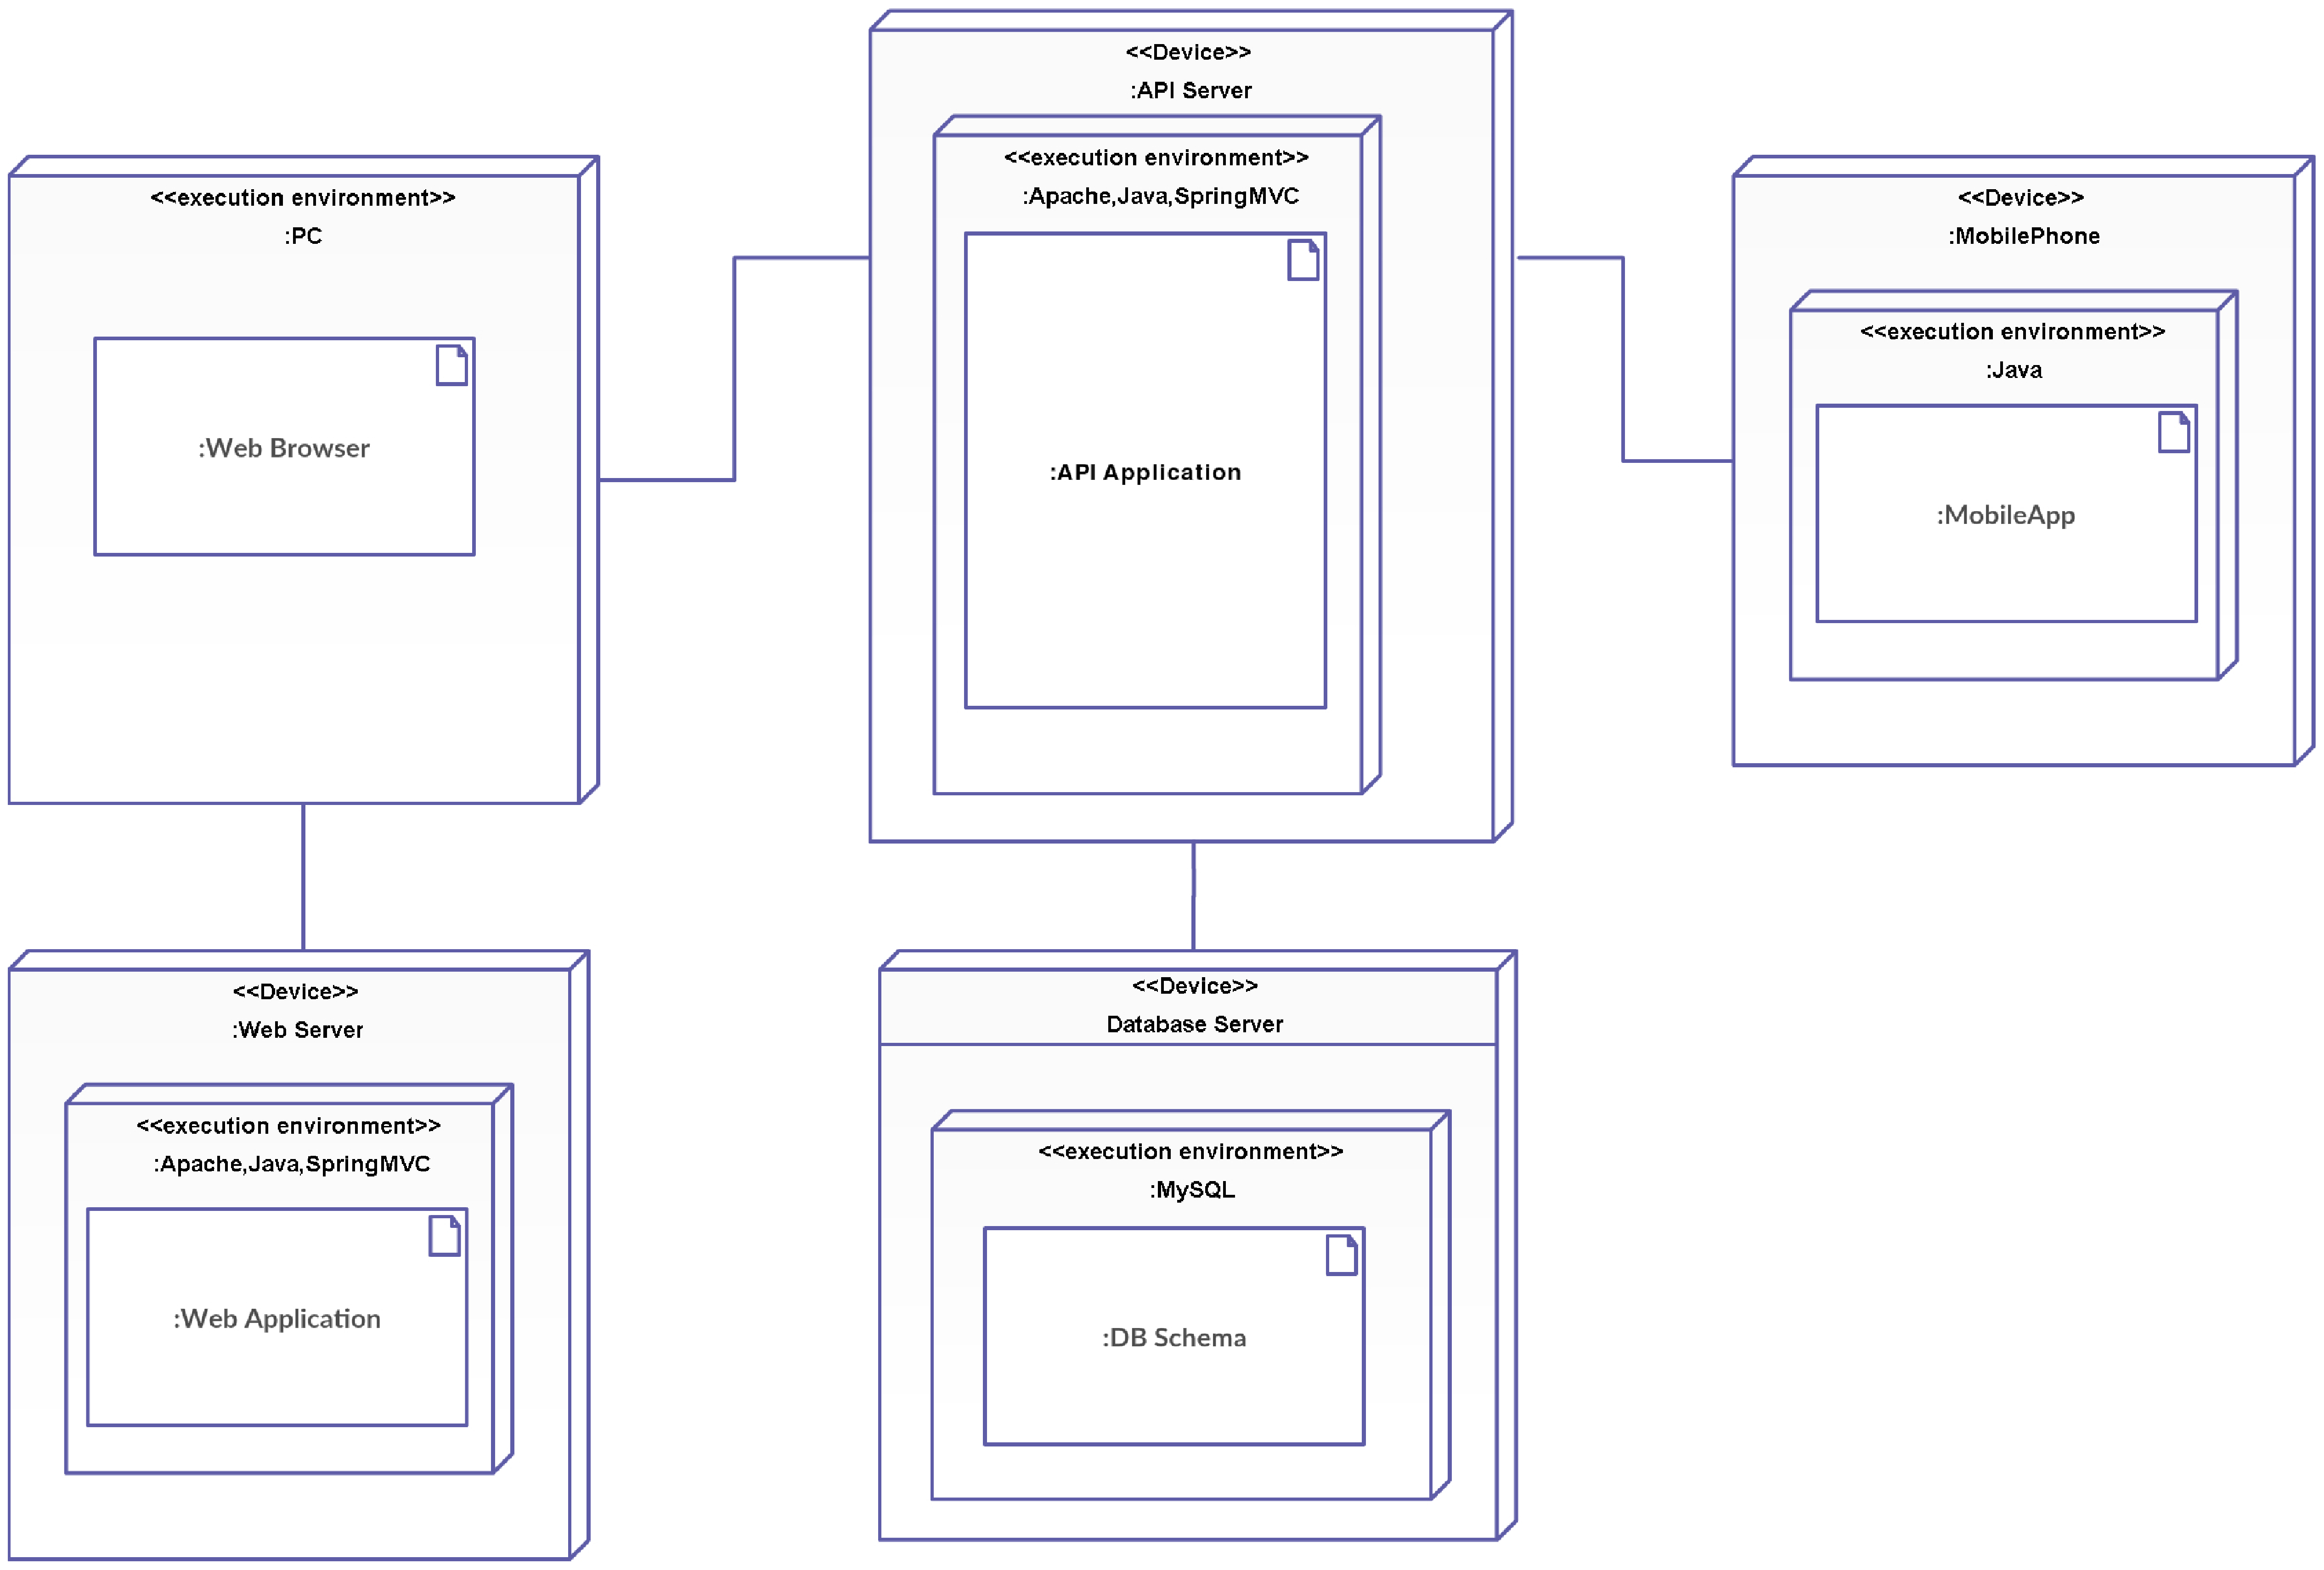
\includegraphics[height=7cm,keepaspectratio]{figures/deployment_view.eps}
		\label{fig:deployment_view}
	\end{figure}
\end{frame}

\begin{frame}
	\frametitle{Selection of Available Car}
	\begin{figure}[H]
		\centering
		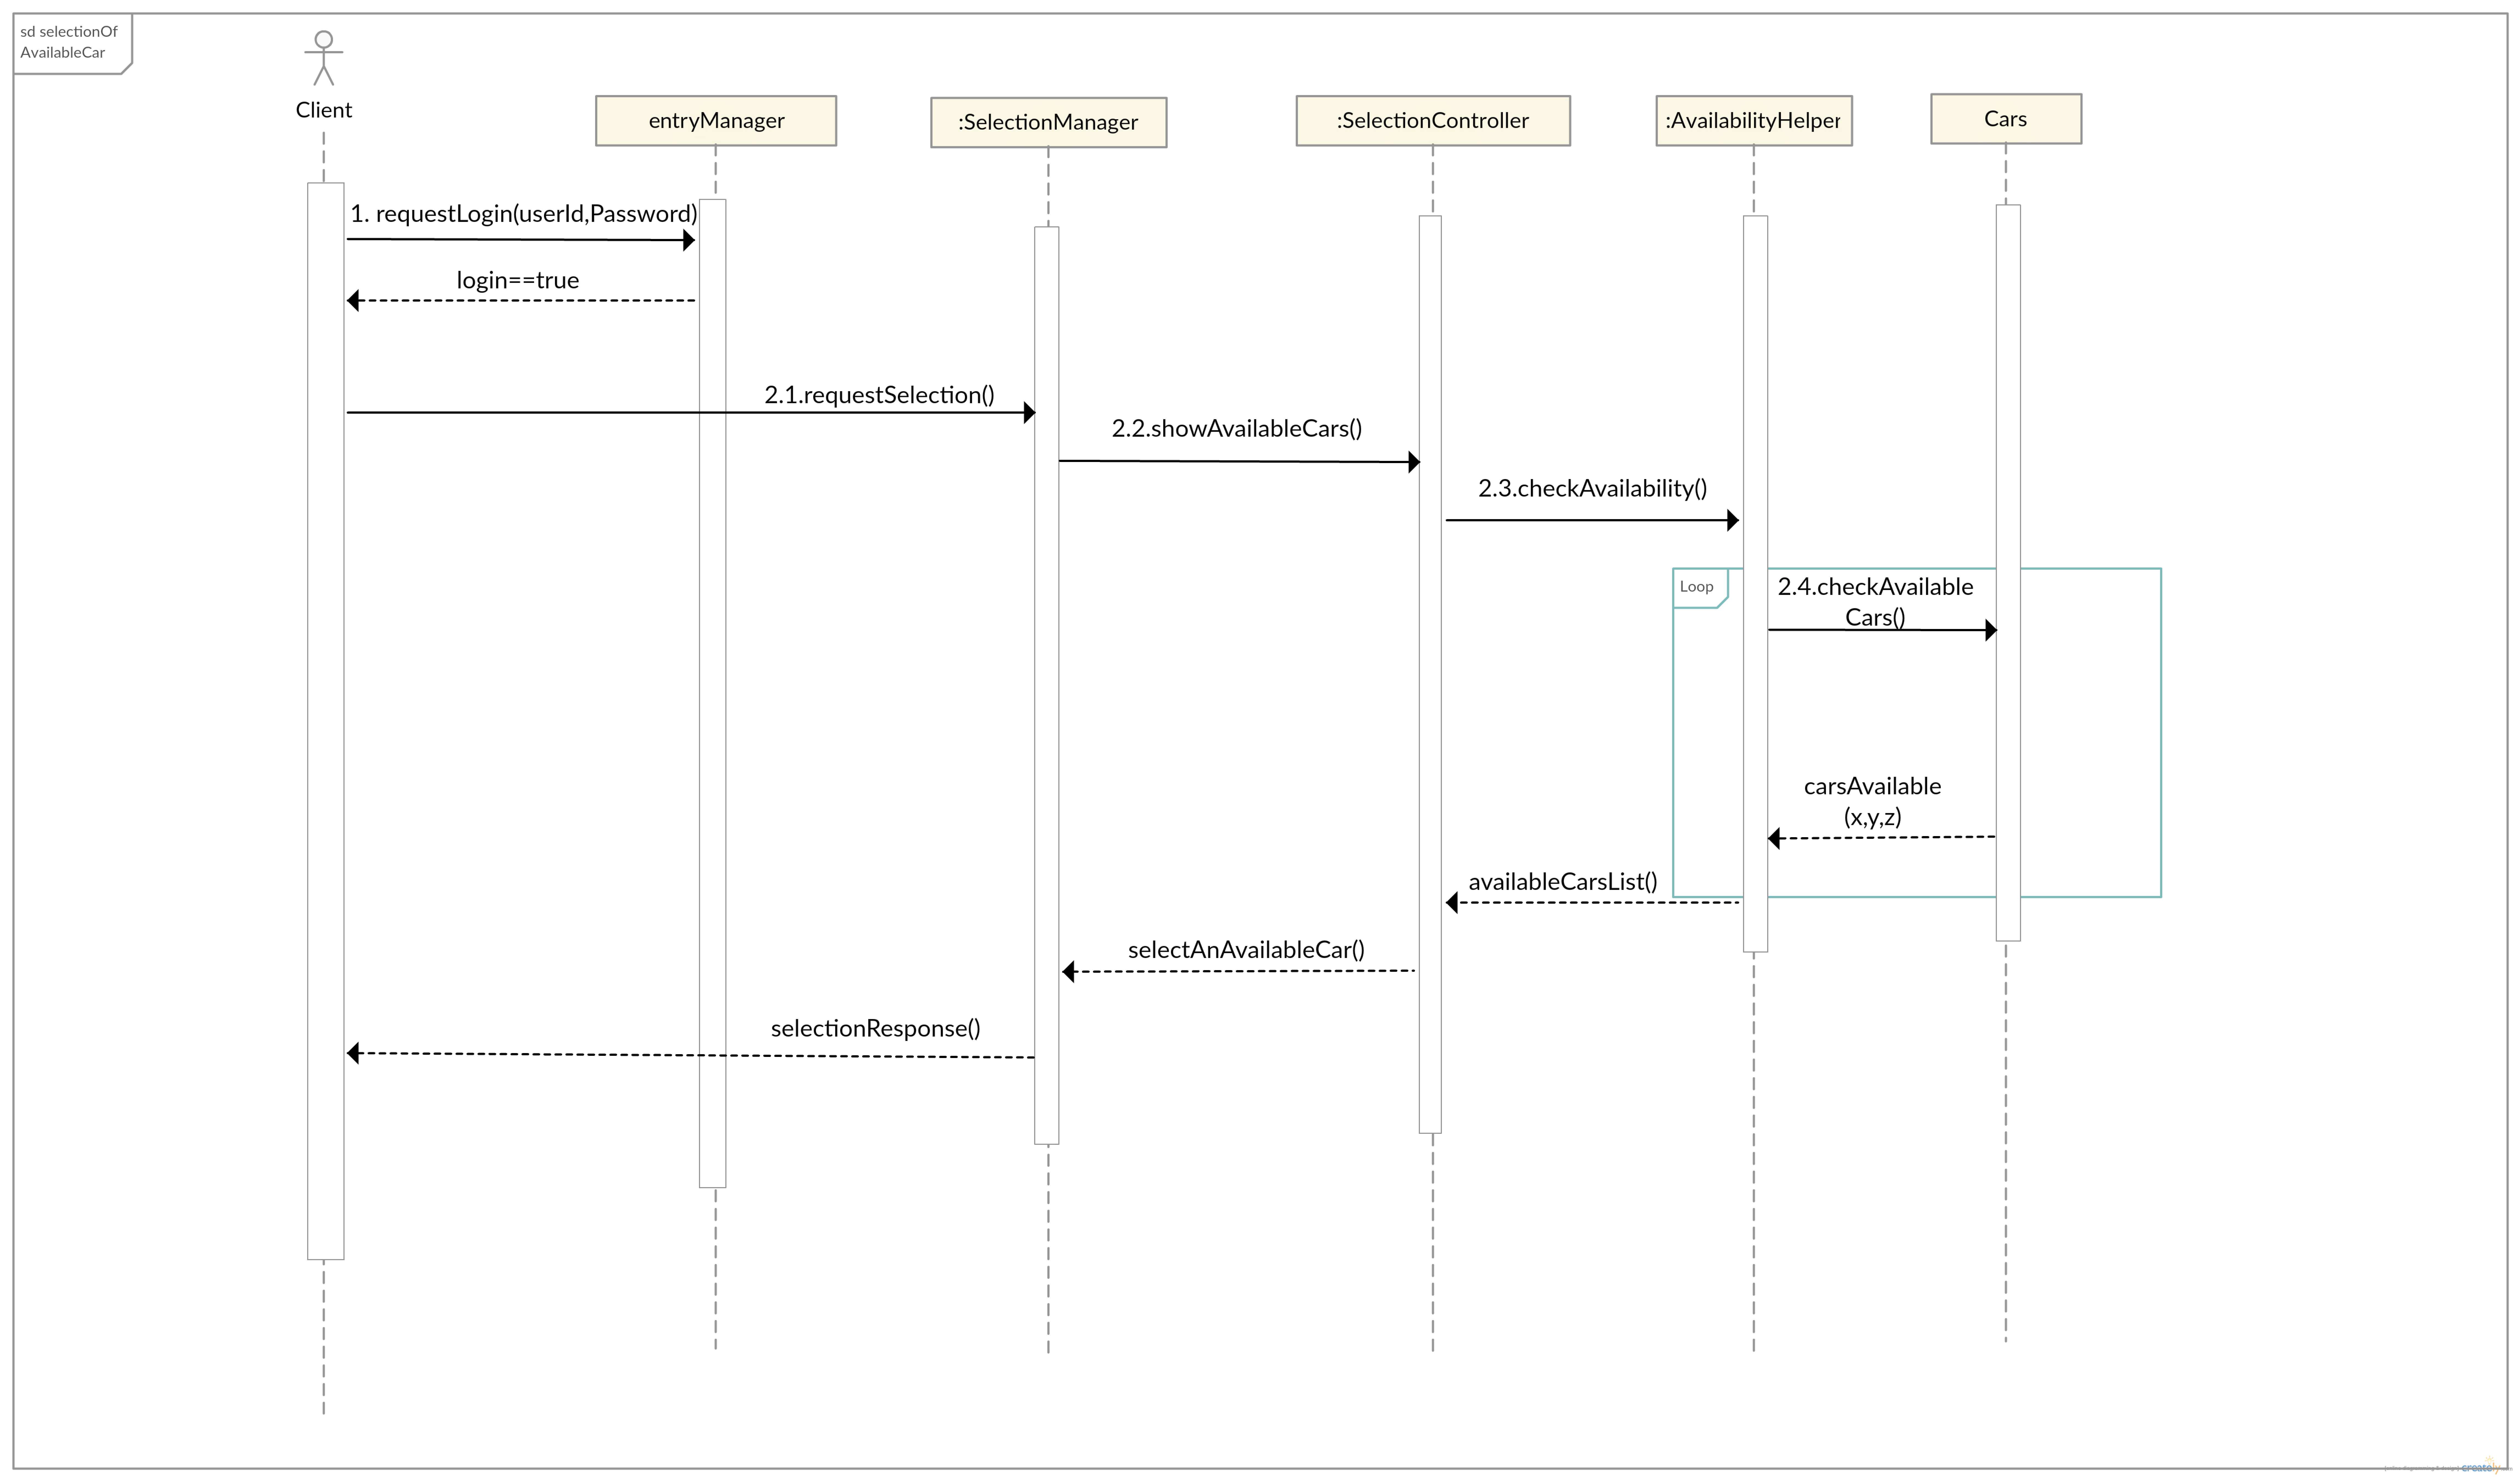
\includegraphics[height=7cm,keepaspectratio]{figures/selection_available_car_runtime.eps}
		\label{fig:selection_available_car}
	\end{figure}
\end{frame}

\begin{frame}
	\frametitle{Reservation of Selected Car}
	\begin{figure}[H]
		\centering
		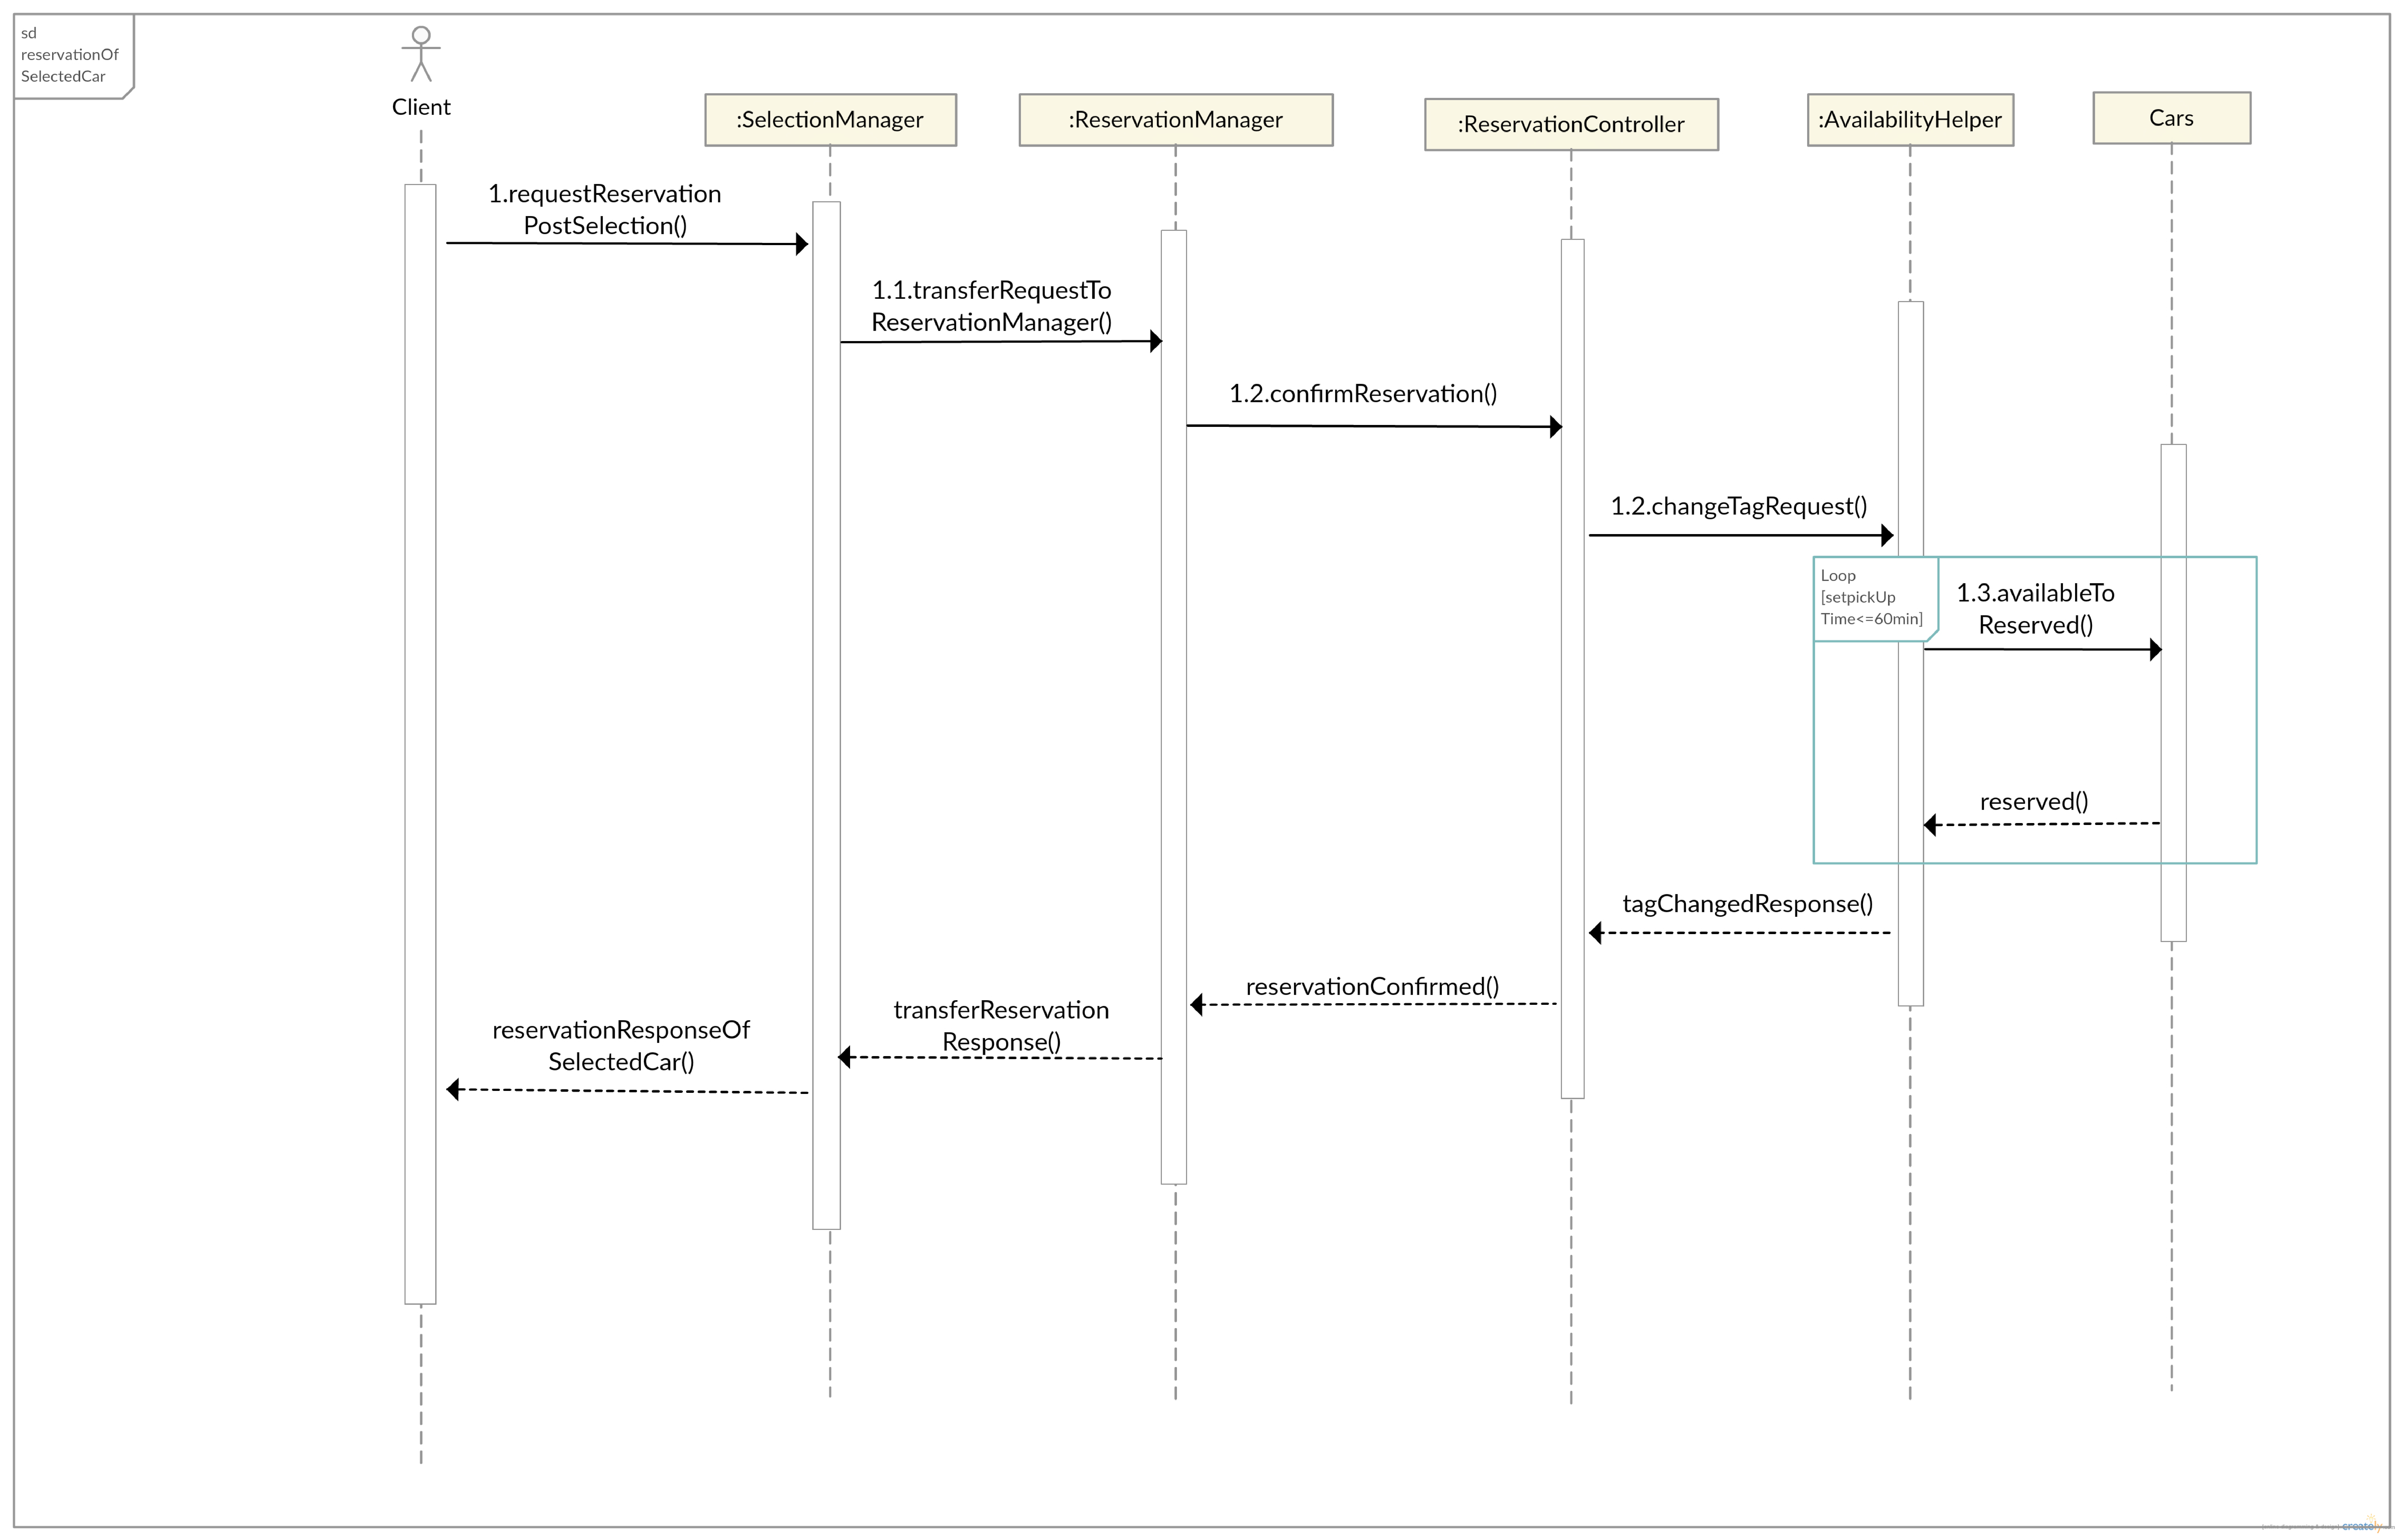
\includegraphics[height=7.3cm,keepaspectratio]{figures/reservation_runtime.eps}
		\label{fig:reservation_runtime}
	\end{figure}
\end{frame}

\begin{frame}
	\frametitle{UX Diagrams}
	\begin{columns}[c]
		\column{.3\textwidth}
		\begin{figure}[H]
			\centering
			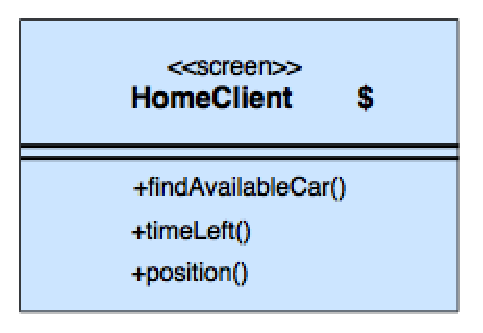
\includegraphics[height=2cm,keepaspectratio]{figures/resv_ux_diagram.eps}
			\label{fig:resv_ux_diagram}
		\end{figure}
		\column{.7\textwidth}
		\begin{figure}[H]
			\centering
			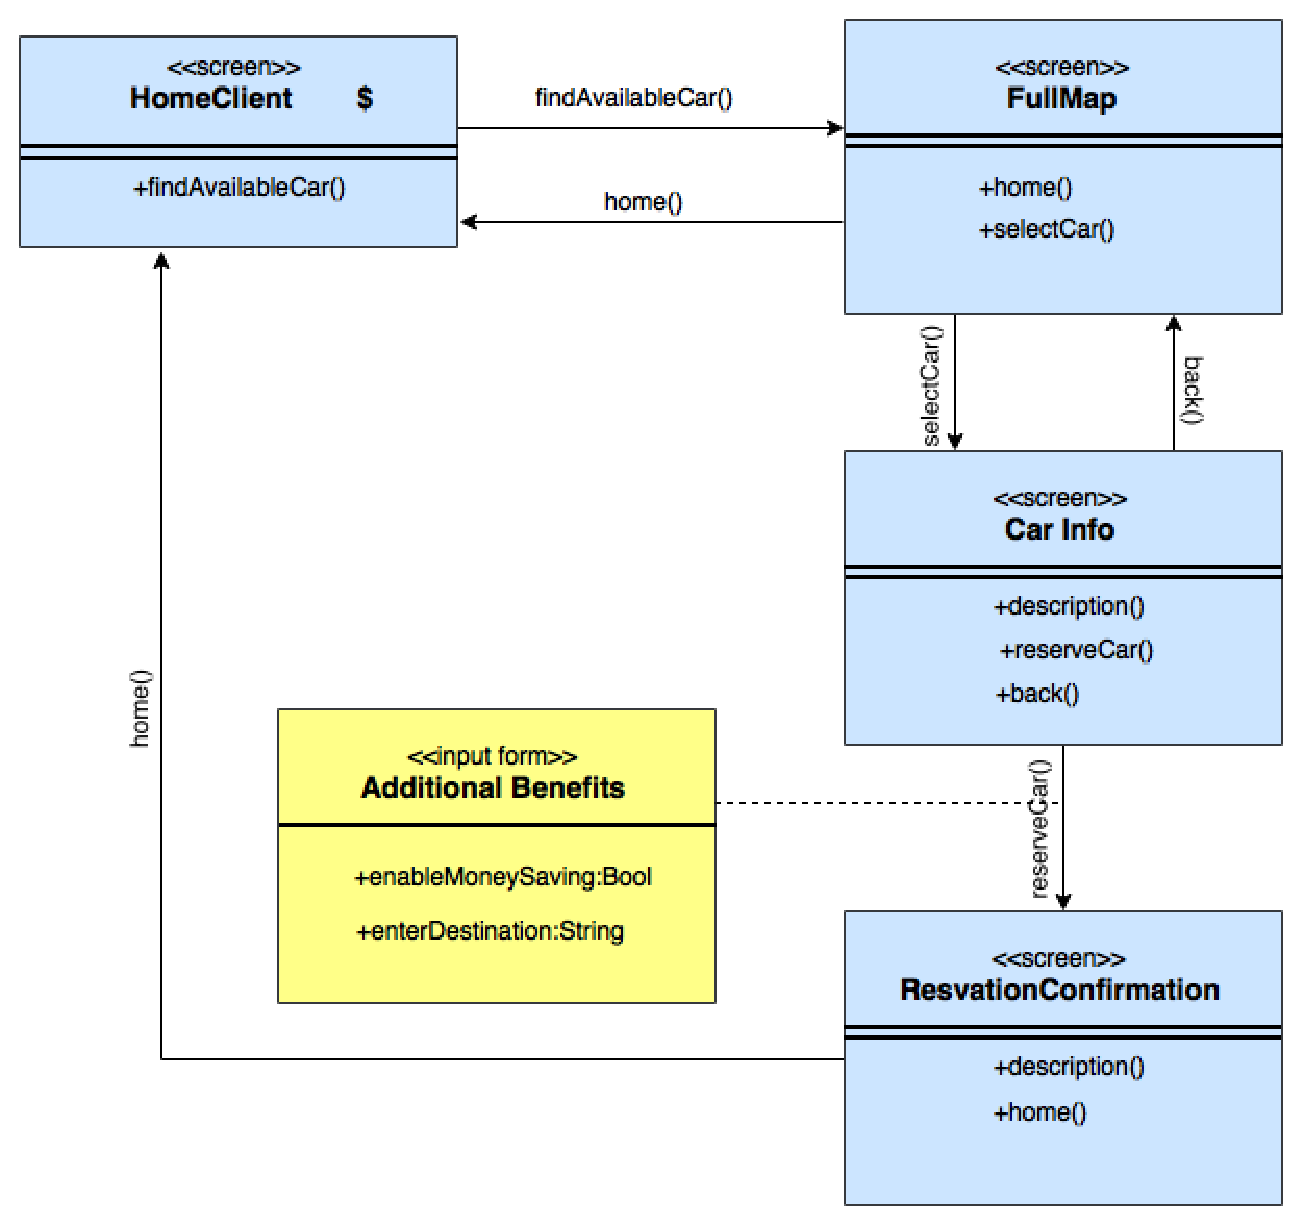
\includegraphics[height=7.3cm,keepaspectratio]{figures/notresv_ux_diagram.eps}
			\label{fig:notresv_ux_diagram}
		\end{figure}
	\end{columns}
\end{frame}
\section{Integration Test Plan Document}

\begin{frame}
	\frametitle{Entry Criteria}
	\begin{itemize}
		\item RASD and DD documents are completely composed
		\item Development goes forward along with their unit testing
		\item Every component has at least 90\% of its functionalities completed
		\item The integration process starts at the achievement of the following percentages of development:
		\begin{itemize}
			\item 100\% of the Database and Availability Helper components
			\item at least 80\% of the Controller components
			\item at least 50\% for the client applications
		\end{itemize}
	\end{itemize}
\end{frame}

\begin{frame}
	\frametitle{Integration testing strategy}
	\qquad \textbf{Bottom-up approach}
	\begin{itemize}
		\item Components integrated from the most independent to the less one
		\item Avoiding useless stubs
		\item Creation of an integrated subsystem
		\item Allowing developers to perform integration testing earlier in the development process
		\item Parallelism and efficiency are maximized
	\end{itemize}
\end{frame}

\begin{frame}
	\frametitle{Components}
	\vspace*{-0.5cm}
	\begin{figure}[H]
		\centering
		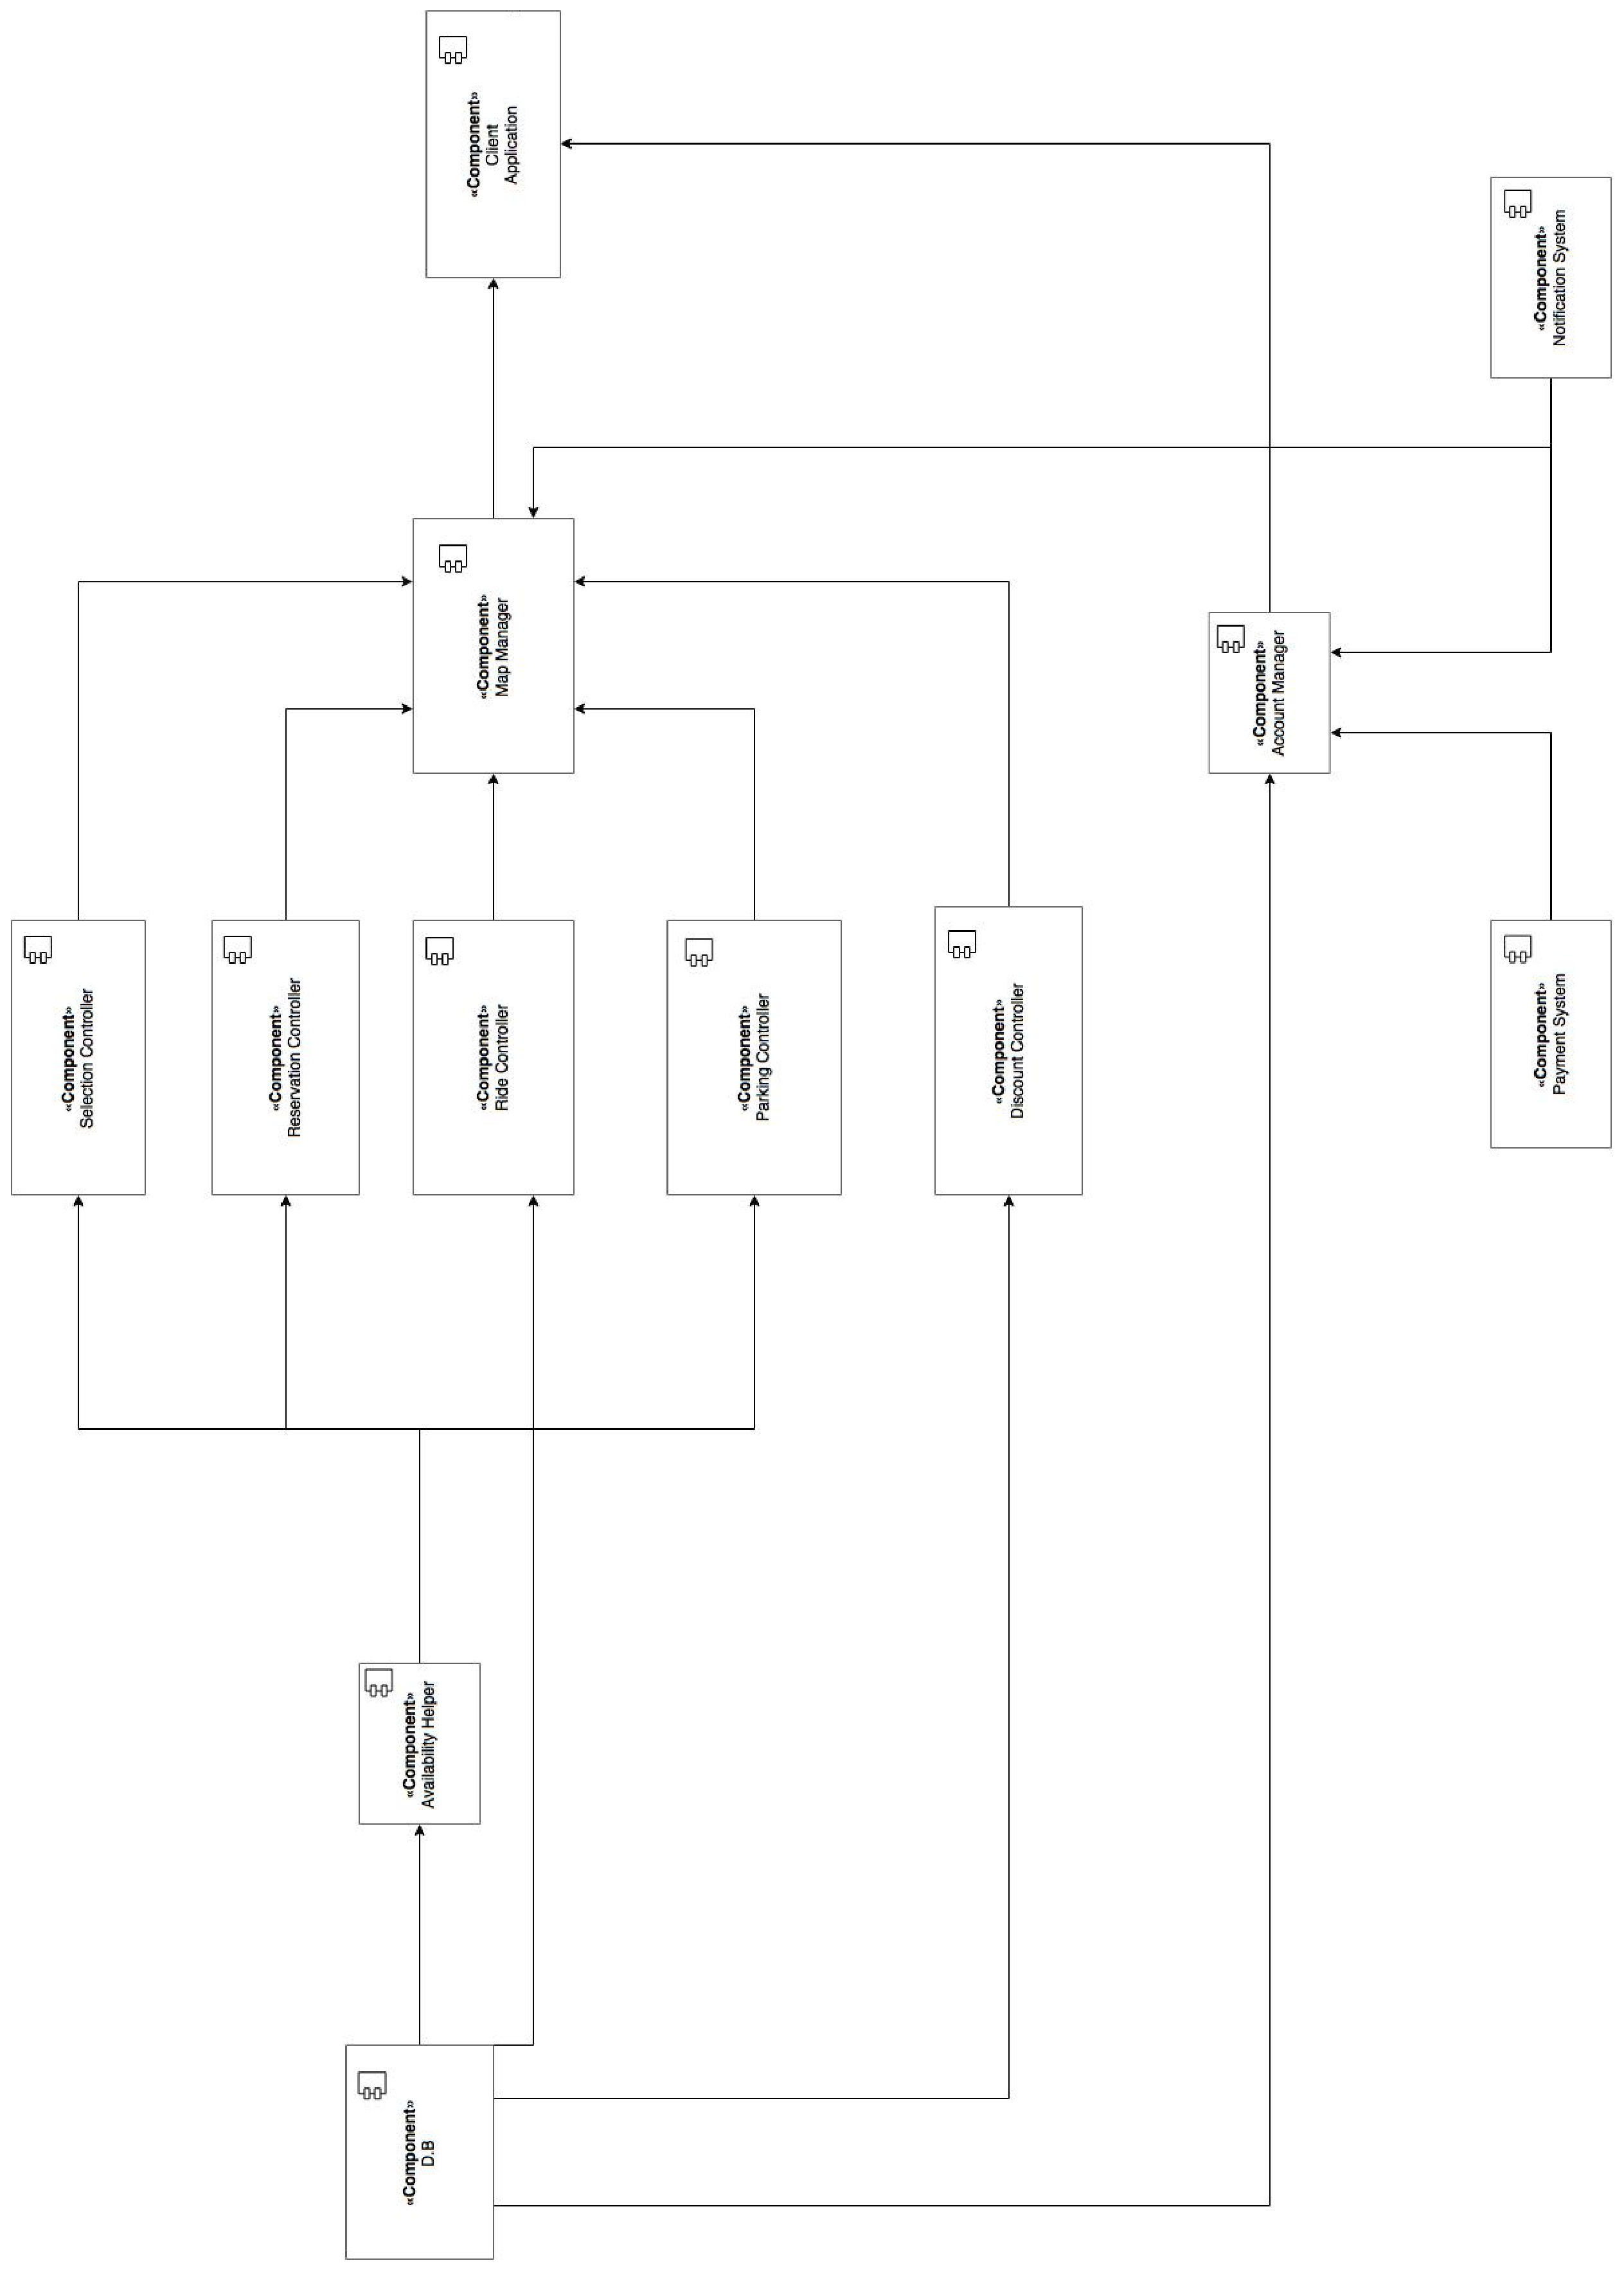
\includegraphics[height=10.5cm,keepaspectratio,angle=270]{figures/components_controller.eps}
		\label{fig:components_controller}
	\end{figure}
\end{frame}

\begin{frame}
	\frametitle{Integration Test Cases}
	\begin{table}[H]
		\centering
		\begin{tabular*}{\textwidth}{p{4.4cm} @{\extracolsep{0.5cm}} p{8.5cm}}
			\hline
			\textbf{Test case identifier} & I5T2 \\
			\hline
			\textbf{Test item(s)} & Reservation Controller \(\rightarrow\) Map Manager \\
			\hline
			\textbf{Input specification} & Post a ReservationController request \\
			\hline
			\textbf{Output specification} & Check if the request is correctly routed \\
			\hline
			\textbf{Environmental needs} & I1, I2, I3 succeeded \\
			\hline
		\end{tabular*}
	\end{table}
	\begin{table}[H]
		\centering
		\begin{tabular*}{\textwidth}{|p{4.0cm}|p{7.18cm}|}
			\hline	
			\multicolumn{2}{|c|}{placeReservation(car) returns response} \\
			\hline
			\textit{Input} & \textit{Effect} \\
			\hline
			A valid car & ReservationController will invoke AvailabilityHelper.changeTagRequest() and get the response R. R is then returned. \\
			\hline
			A null or invalid car & A NullCarException or InvalidCarException is generated. \\
			\hline
		\end{tabular*}
	\end{table}
\end{frame}

\begin{frame}
	\frametitle{Program Stubs}
	\begin{itemize}

		\item Reduced number of drivers is required to perform necessary method invocations
		\begin{itemize}
			\item \emph{AvailabilityHelper driver}: invokes the methods exposed by the component AvailabilityHelper in order to test its interaction with the database management system
			\item \emph{Controllers driver}: invokes the methods exposed by the Controllers (acting like MapManager) in order to test its interaction with each other
		\end{itemize}
		\item Only one stub acting like the client to fulfill the request/response protocol during client/system interaction
	\end{itemize}
\end{frame}

\end{document}